\documentclass[11pt]{report}
\usepackage[utf8]{inputenc}
\usepackage[italian]{babel}
\usepackage{hyperref}
\usepackage{url}
\usepackage{natbib}
\usepackage{graphicx}
\usepackage{parskip}
\usepackage{float}

\newcommand{\emailaddr}[1]{\large\href{mailto:#1}{\texttt{#1}}}

\usepackage{listings}
\usepackage{xcolor}

% Define TypeScript language settings
\lstdefinelanguage{TypeScript}{
  morekeywords={typeof, new, true, false, catch, function, return, null, catch, switch, var, if, in, while, do, else, case, break, class, export, async, namespace, const, type, extends},
  morecomment=[l]{//},
  morecomment=[s]{/*}{*/},
  morestring=[b]',
  morestring=[b]",
  sensitive=true
}

% Define code listing style
\lstdefinestyle{typescript}{
  language=TypeScript,
  basicstyle=\ttfamily\small,
  keywordstyle=\color{blue},
  commentstyle=\color{gray},
  stringstyle=\color{purple},
  numbers=left,
  numberstyle=\tiny,
  stepnumber=1,
  numbersep=5pt,
  backgroundcolor=\color{white},
  frame=single,
  breaklines=true,
  breakatwhitespace=true,
  tabsize=2
}

%%%%%%%%%%%%%%%%%%%%%%%%%%%%%%%%%%%%%%%%%%%%%%%%%%%%%%
%%%%%%%%%%% YAML syntax highlighting %%%%%%%%%%%%%%%%%

% http://tex.stackexchange.com/questions/152829/how-can-i-highlight-yaml-code-in-a-pretty-way-with-listings

% here is a macro expanding to the name of the language
% (handy if you decide to change it further down the road)
\newcommand\YAMLcolonstyle{\color{red}\mdseries}
\newcommand\YAMLkeystyle{\color{black}\bfseries}
\newcommand\YAMLvaluestyle{\color{blue}\mdseries}

\makeatletter

\newcommand\language@yaml{yaml}

\expandafter\expandafter\expandafter\lstdefinelanguage
\expandafter{\language@yaml}
{
  keywords={true,false,null,y,n},
  keywordstyle=\color{darkgray}\bfseries,
  basicstyle=\YAMLkeystyle,                                 % assuming a key comes first
  sensitive=false,
  comment=[l]{\#},
  morecomment=[s]{/*}{*/},
  commentstyle=\color{purple}\ttfamily,
  stringstyle=\YAMLvaluestyle\ttfamily,
  moredelim=[l][\color{orange}]{\&},
  moredelim=[l][\color{magenta}]{*},
  moredelim=**[il][\YAMLcolonstyle{:}\YAMLvaluestyle]{:},   % switch to value style at :
  morestring=[b]',
  morestring=[b]",
  literate =    {---}{{\ProcessThreeDashes}}3
                {>}{{\textcolor{red}\textgreater}}1     
                {|}{{\textcolor{red}\textbar}}1 
                {\ -\ }{{\mdseries\ -\ }}3,
}

% switch to key style at EOL
\lst@AddToHook{EveryLine}{\ifx\lst@language\language@yaml\YAMLkeystyle\fi}
\makeatother

\newcommand\ProcessThreeDashes{\llap{\color{cyan}\mdseries-{-}-}}

%%%%%%%%%%% YAML syntax highlighting %%%%%%%%%%%%%%%%%
%%%%%%%%%%%%%%%%%%%%%%%%%%%%%%%%%%%%%%%%%%%%%%%%%%%%%%

\title{
    Piperchat \\
    \large Applicazioni e Servizi Web
}

\author{ \Large
    Alessandro Mazzoli \\ \emailaddr{alessandro.mazzoli9@studio.unibo.it}
    \and \Large
    Luigi Borriello \\ \emailaddr{luigi.borriello2@studio.unibo.it} 
    \and \Large
    Tommaso Patriti \\ \emailaddr{tommaso.patriti@studio.unibo.it}
}
\date{\today}



\begin{document}

\maketitle

\tableofcontents

\chapter{Introduzione}

Il progetto consiste nella realizzazione di una piattaforma che permette la comunicazione fra gli utenti, ispirata a \href{https://discord.com}{Discord}.

Piperchat, mira a creare un ambiente di comunicazione ispirato a Discord, dove gli utenti possono interagire in varie forme.
%
Offrirà la possibilità di registrazione e accesso tramite un sistema di login, consentendo agli utenti di stabilire e gestire connessioni sociali attraverso richieste di amicizia.
%
La piattaforma faciliterà la comunicazione intra-utente, con notifiche per messaggi e la gestione delle amicizie.
%
Gli utenti avranno la libertà di creare e gestire i propri server, con funzionalità per la gestione di canali testuali e multimediali.
%
Sarà possibile inviare messaggi, partecipare a chiamate vocali e video e gestire webcam e microfono all'interno dei canali.
%
Inoltre, i creatori dei server potranno moderarli, rimuovendo membri indesiderati.


\chapter{Requisiti}
\section{Funzionali}

\begin{itemize}
    \item \textbf{Registrazione e Autenticazione}:
    \begin{itemize}
        \item Possibilità di registrazione al sistema.
        
        \item Possibilità di login nel sistema.
    \end{itemize}
    \item \textbf{Sistema di amicizie}:
    \begin{itemize}
        \item Possibilità di inviare richieste di amicizia.
        
        \item Possibilità di accettare o rifiutare richieste di amicizia.
        
        \item Sistema di notifiche per la ricezione di nuovo richieste di amicizia.
        
        \item Sistema di gestione dello stato e dell'ultimo accesso degli utenti.
    \end{itemize}
    \item \textbf{Messaggistica Infra-Utente}:
    \begin{itemize}
        \item Gestione messaggistica tra amici
        
        \item Sistema di notifiche per l'arrivo di nuovi messaggi.
    \end{itemize}
    \item \textbf{Gestione Server}:
    \begin{itemize}
        \item Possibilità di creazione di un nuovo server.
        
        \item Possibilità di join di un server esistente.
        
        \item Possibilità da parte del creatore del server di rimozione dei membri.
    \end{itemize}
    \item \textbf{Gestione canali testuali}:
    \begin{itemize}
        \item Possibilità di creazione di canali testuali da parte dell'owner del server.
        \item Possibilità di rimozione di canali testuali da parte dell'owner del server.
        \item Sistema di messaggistica per i canali testuali
        \item Sistema di notifiche per i nuovi messaggi inviati all'interno di canali testuali.
    \end{itemize}
    \item \textbf{Gestione canali multimediali}:
    \begin{itemize}
        \item Possibilità di creazione di canali multimediali da parte dell'owner del server.
        \item Possibilità di rimozione di canali multimediali da parte dell'owner del server.
        \item Sistema di videochiamate.
        \item Gestione della webcam e del microfono.
    \end{itemize}
\end{itemize}

\section{Requisiti non Funzionali (Usabilità e Accessibilità)}
\begin{itemize}
    \item \textbf{Sistema di monitoring dei microservizi}:
    \begin{itemize}
        \item Sistema di monitoraggio dello stato dei servizi.
        \item Dashboard per visualizzare lo stato real-time dei servizi.
    \end{itemize}
    
    \item \textbf{Supporto temi}: l'applicazione deve poter gestire il cambio di tema, offrendo anche un opzione a supporto di utenti con dislessia.
    
    \item \textbf{Test di Accessibilità}: Prima del rilascio ufficiale, l'applicazione deve essere sottoposta a test di accessibilità per identificare e correggere eventuali problemi relativi all'accessibilità.
\end{itemize}




\chapter{Design}

Il progetto è stato guidato da un modello iterativo basato sullo \textbf{User Centered Design}.
%
Inizialmente, sono stati definiti gli utenti target dell'applicazione, sui quali sono state create le \textit{Personas}.
%
Queste ultime hanno svolto un ruolo cruciale nello sviluppo e nella comprensione delle funzionalità del sistema, garantendo un adattamento ai requisiti degli utenti.

Come processo di sviluppo abbiamo adottato una metodologia simile all'Agile, in cui sono state frequentemente analizzate le attività da svolgere e le relative priorità, così come il carico di lavoro assegnato e i feedback sul lavoro svolto.
%
Lato frontend, le interfacce utente sono state progettate secondo i principi fondamentali del design:

\begin{itemize}
    \item il \textbf{KISS} (Keep It Simple, Stupid) per garantire un'esperienza priva di complicazioni e ridurre al minimo gli errori degli utenti durante la navigazione nell'applicazione.
    \item Sono stati impiegati i principi del Responsive Design come base per garantire un elevato livello di usabilità dell'applicazione.
\end{itemize}

%
%
%
\section{Target User Analisys}

Nel processo di progettazione del nostro sistema, abbiamo identificato diversi profili di utenti per comprendere meglio le esigenze e i comportamenti dei potenziali fruitori del nostro servizio.

%
%
%
\subsection{Personas 1: Il Gamer}

\textbf{Nome:} Luca

\textbf{Età:} 23

\textbf{Occupazione:} Studente universitario e appassionato di videogiochi

\textbf{Obiettivi e Comportamenti:} Luca è un giocatore accanito che trascorre molte ore al giorno giocando a una varietà di giochi online. Cerca una piattaforma come la nostra per connettersi con altri giocatori, formare squadre e partecipare a sessioni di gioco cooperative. È interessato a funzionalità quali chat vocali durante il gioco, organizzazione di eventi e discussioni sui giochi più popolari. La sua priorità è un'interfaccia semplice e reattiva per facilitare la sua partecipazione e l'organizzazione di eventi di gioco.

%
%
%
\textbf{Personas 2: Elisa - L'appassionata di Lettura e Libri}

\textbf{Età:} 35

\textbf{Occupazione:} Libraia e Blogger

\textbf{Obiettivi e Comportamenti:} Elisa è appassionata di libri e gestisce un blog letterario. Cerca una piattaforma per connettersi con altri lettori, organizzare club del libro online e discutere di opere letterarie. Desidera una piattaforma con chat testuali, possibilità di creare gruppi tematici dedicati ai diversi generi letterari e strumenti per organizzare eventi come letture collettive e sessioni di discussione.

%
%
%
\subsection{Personas 3: Lo Studente Organizzato}

\textbf{Nome:} Giada

\textbf{Età:} 19

\textbf{Occupazione:} Studentessa universitaria

\textbf{Obiettivi e Comportamenti:} Giada è una studente impegnata che cerca un'interfaccia per connettersi con altri studenti, partecipare a discussioni relative ai corsi e organizzare gruppi di studio. Desidera un'esperienza di messaggistica testuale intuitiva e efficiente che le consenta di partecipare attivamente alle conversazioni relative alle sue lezioni e argomenti di studio. La possibilità di effettuare videochiamate per discussioni di gruppo o sessioni di studio è un aspetto cruciale per lei. Un'interfaccia pulita e facile da usare, specialmente su dispositivi mobili, è essenziale per supportare il suo coinvolgimento attivo nell'apprendimento collaborativo.

%
%
%
\subsection{Riflessioni}

La creazione di queste tre diverse personas ci ha permesso di visualizzare in modo più tangibile e realistico i diversi tipi di utenti che potrebbero utilizzare la piattaforma. Questa analisi ci ha guidato nella progettazione di funzionalità e caratteristiche mirate a soddisfare le esigenze specifiche di ciascun tipo di utente identificato.

%
%
%
\section{Mockup}
Durante la fase di design, è stato utilizzato Figma per la realizzazione di una serie di mockup, nei quali abbiamo testato, diverse combinazioni cromatiche, trovando così le più appropiate per la nostra applicazione.
\\
%
Utilizzando i suoi strumenti, abbiamo potuto esaminare e ottimizzare l'impiego degli spazi, valutando le varie disposizioni degli elementi nel design e assicurandoci che l'esperienza dell'utente fosse ottimale in termini di fluidità e accessibilità.

Di seguito riportati i mockup realizzati durante la fase di design:

\begin{figure}[htbp]
    \centering
    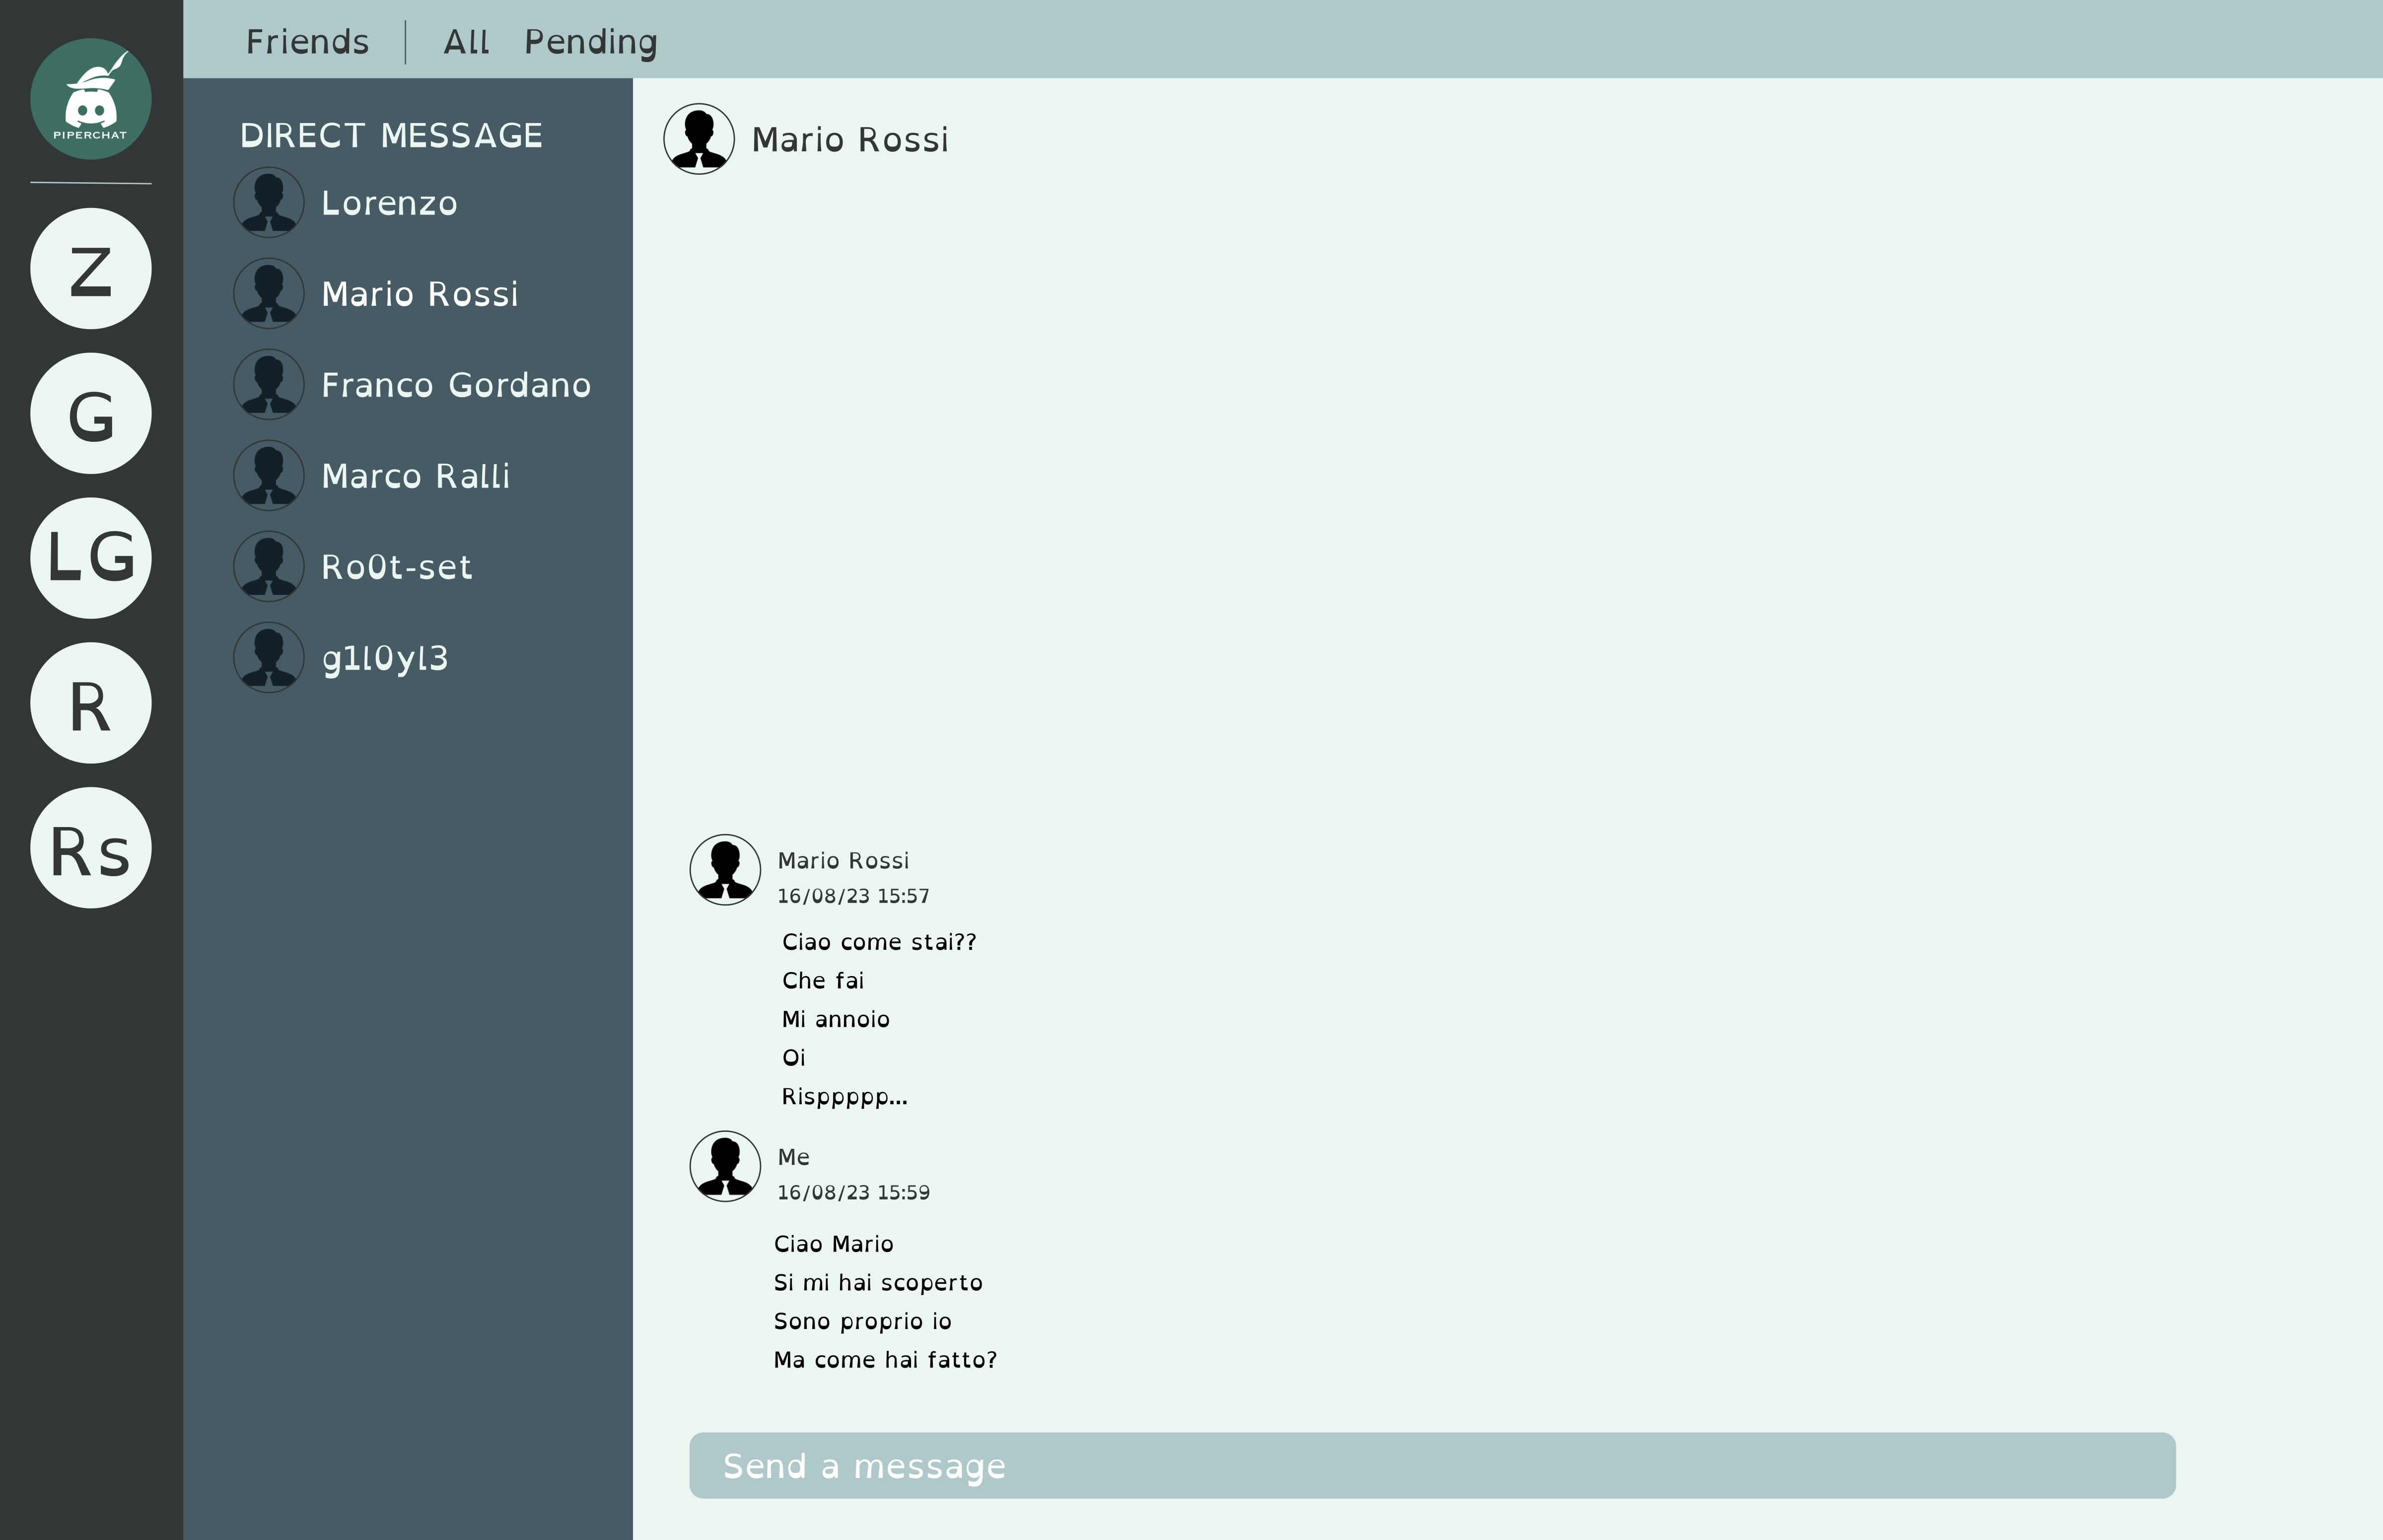
\includegraphics[angle=-90,width=0.92\textwidth]{img/mk2.jpg}
    \caption{Mockup chat}
    \label{fig:mockup2}
\end{figure}

\begin{figure}[htbp]
    \centering
    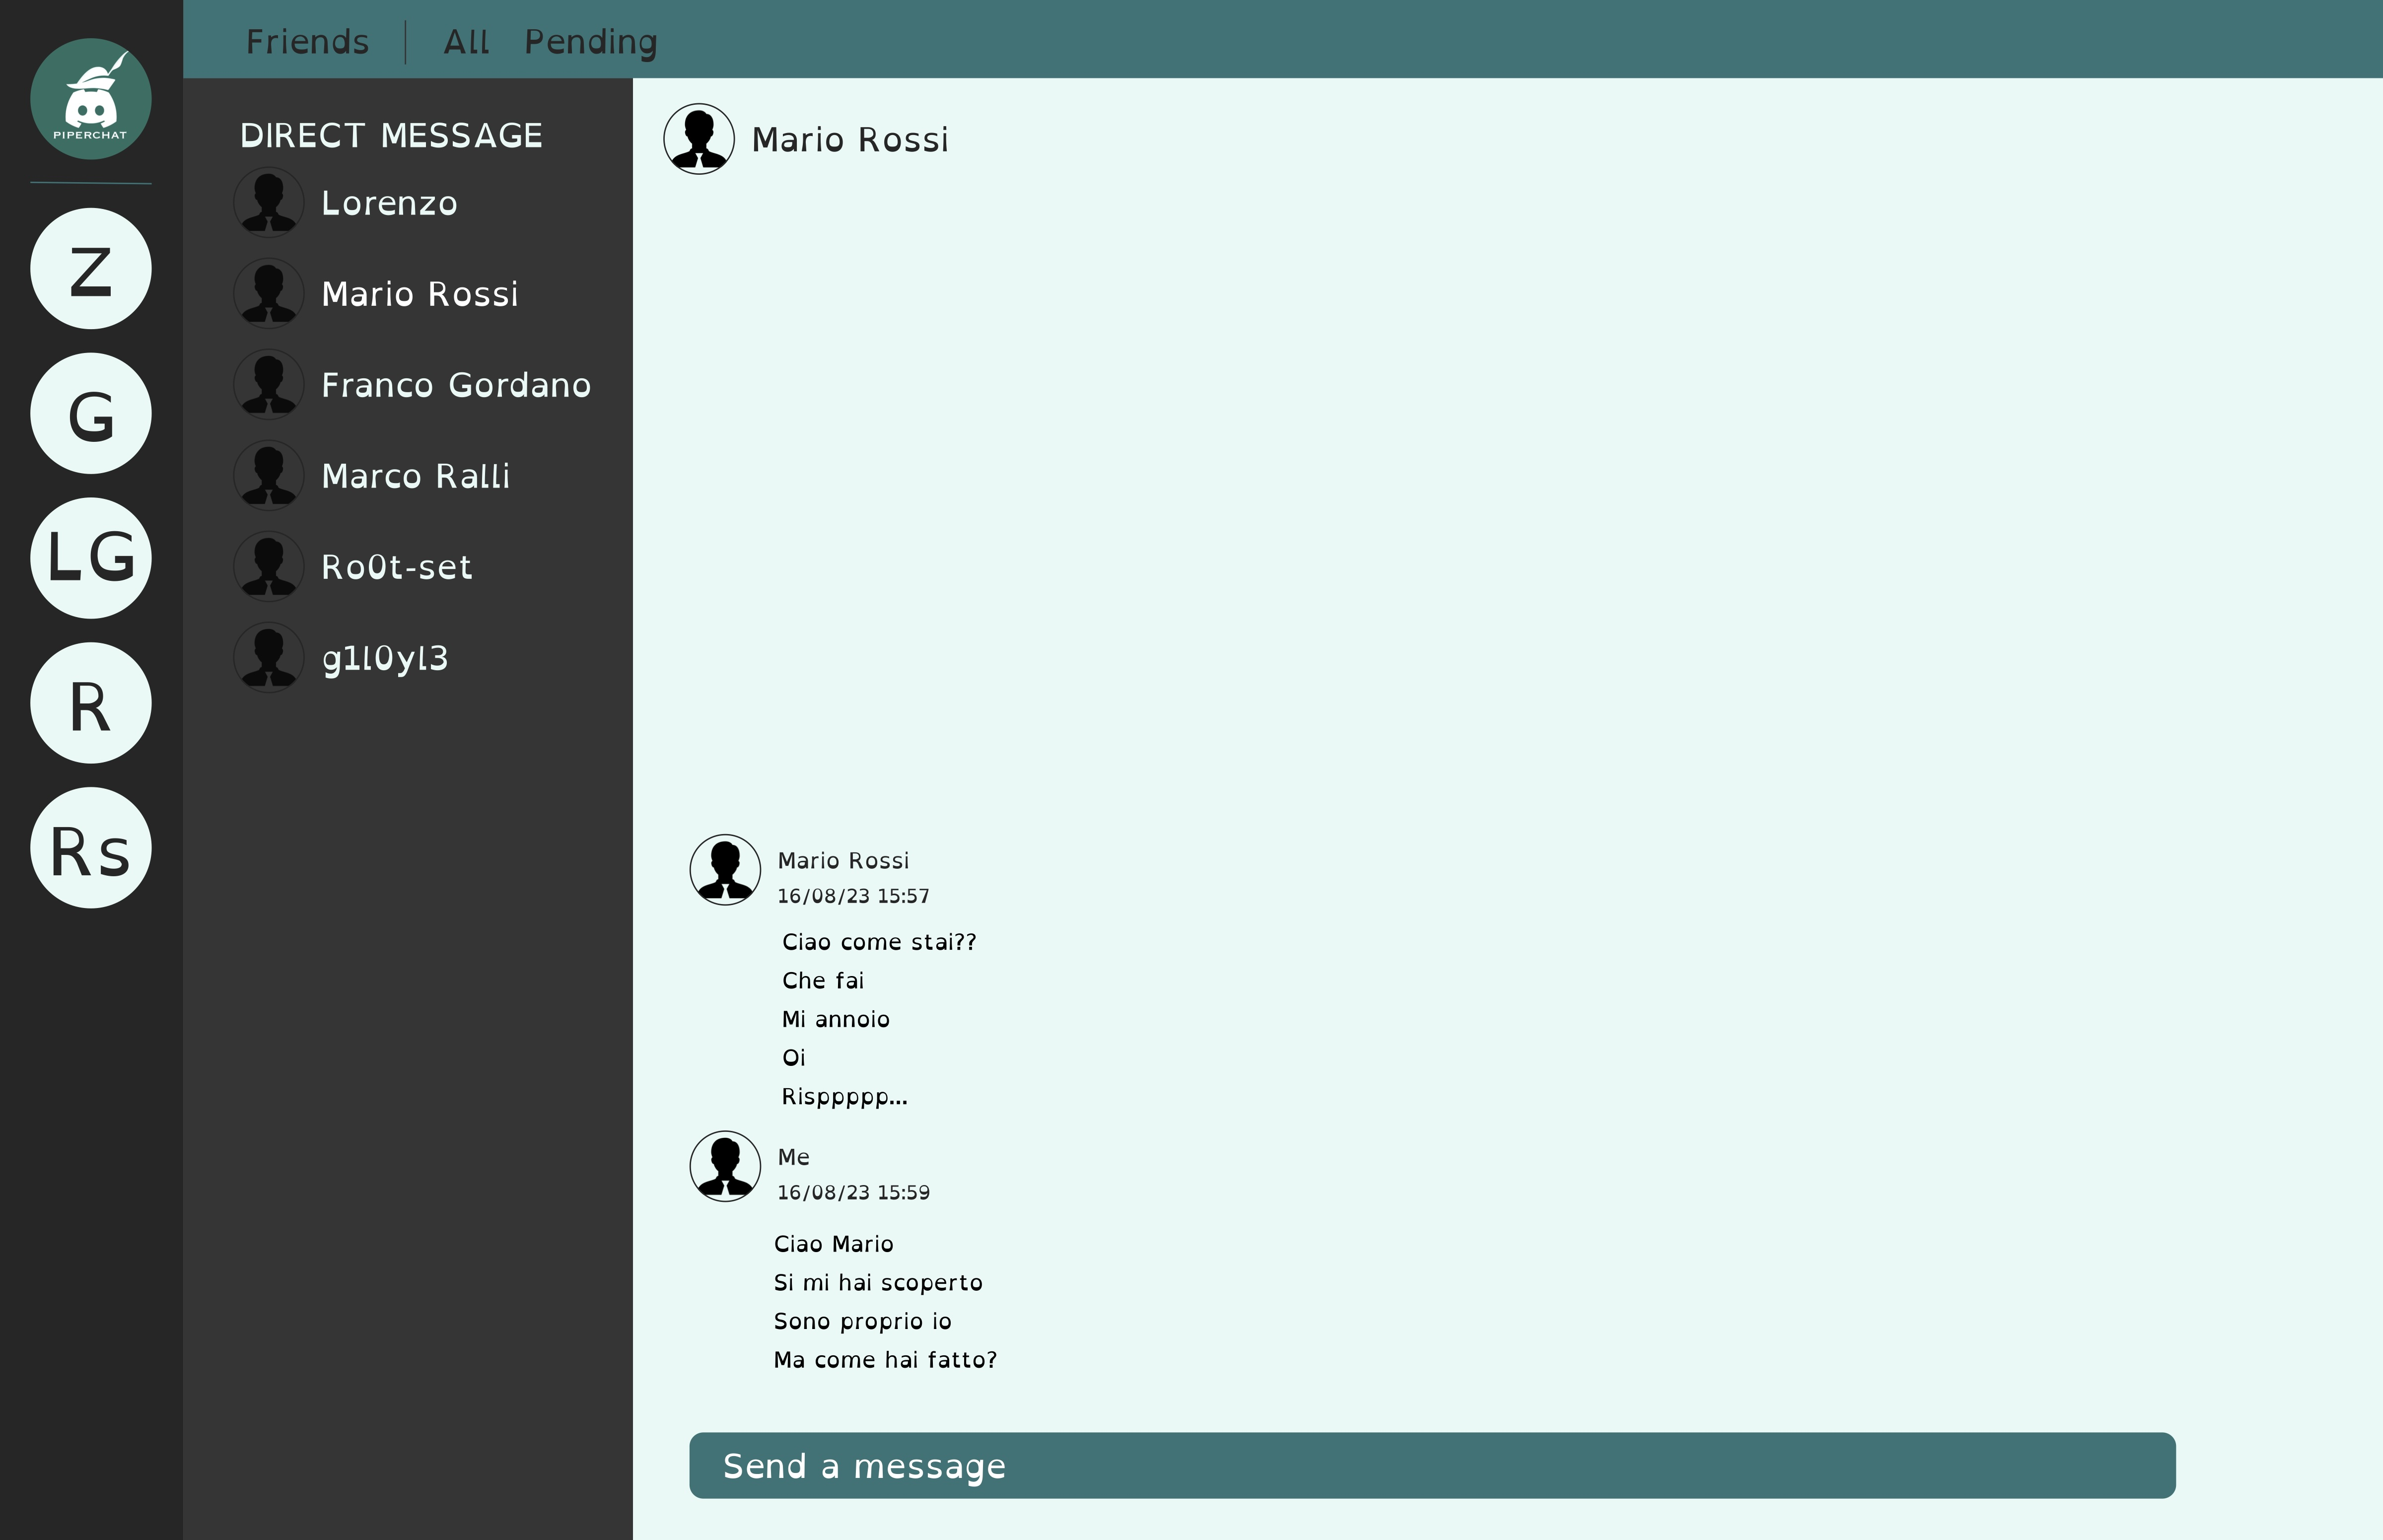
\includegraphics[angle=-90,width=0.92\textwidth]{img/mk3.jpg}
    \caption{Mockup chat con cambio dei colori}
    \label{fig:mockup3}
\end{figure}

\begin{figure}[htbp]
    \centering
    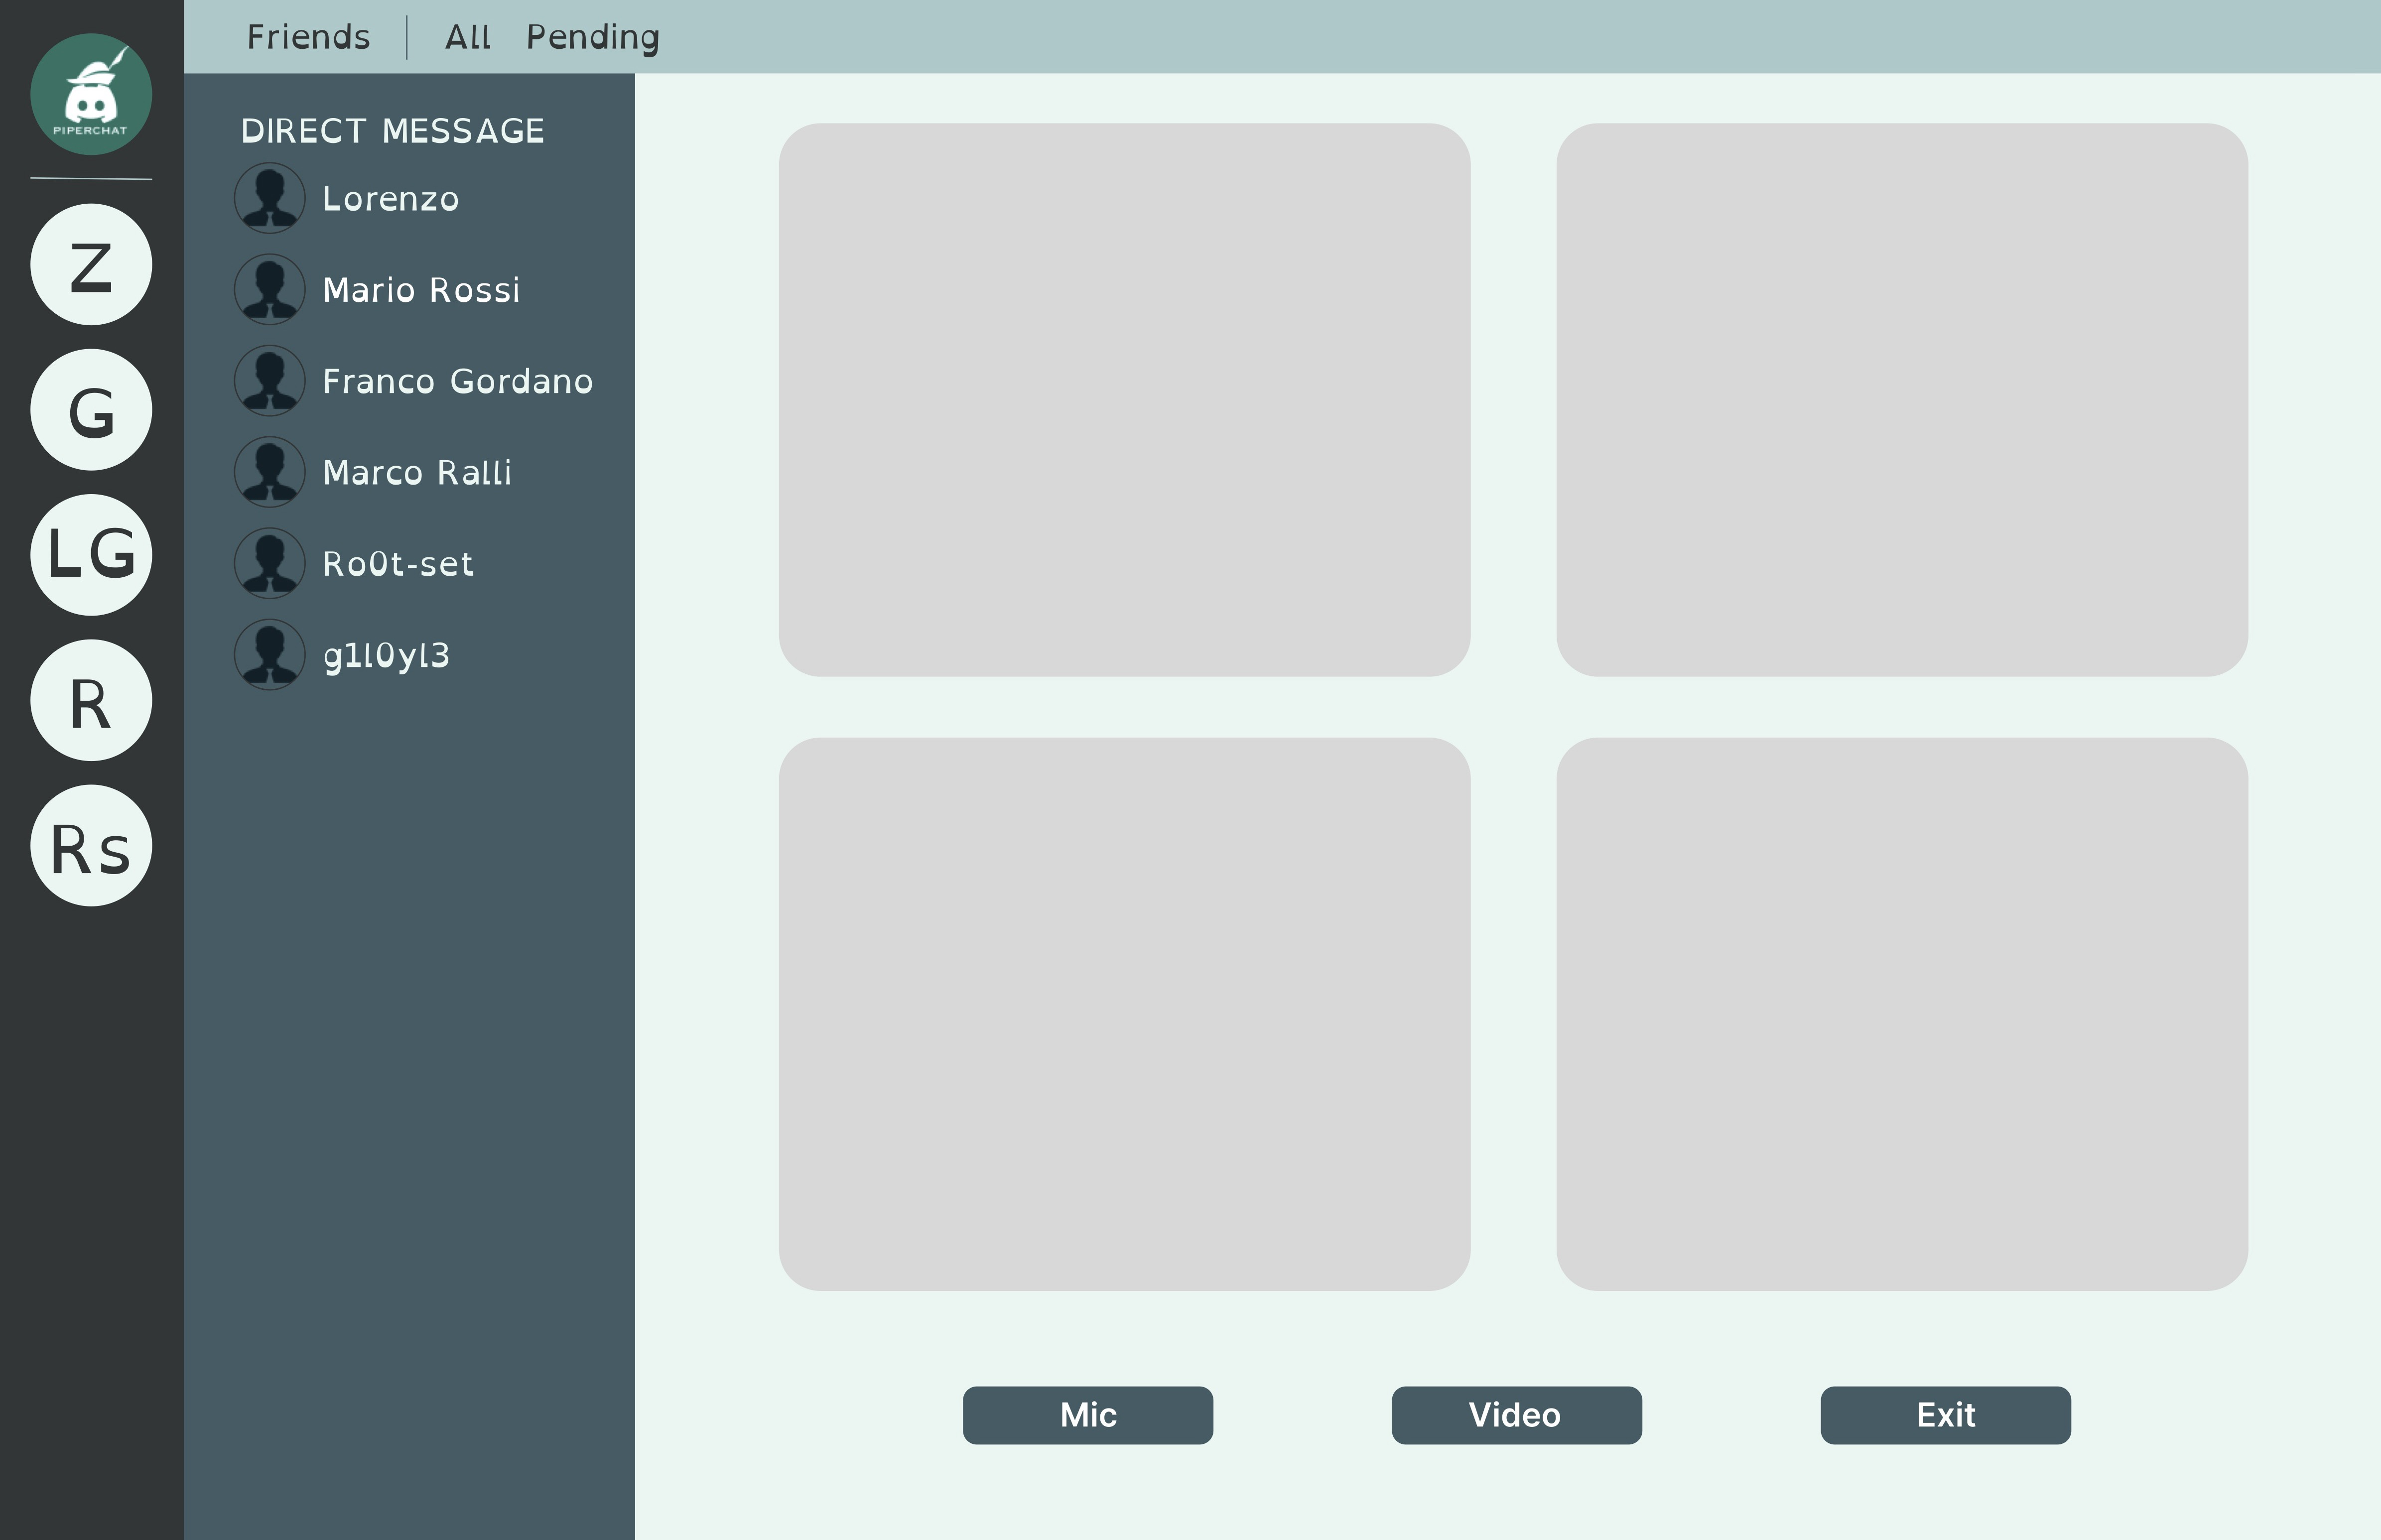
\includegraphics[angle=-90,width=0.92\textwidth]{img/mk4.jpg}
    \caption{Mockup video chat}
    \label{fig:mockup1}
\end{figure}

%
%
%
\newpage
\section{Design Architetturale}

Il sistema è realizzato mediante un'architettura a \emph{microservizi}.
%
Questo permette di suddividere la complessità in parti più piccole, ad alta coesione ed accoppiate in modo lasco.
%
Inoltre, ogni microservizio, se necessario, dispone di un \emph{database}, al quale può accedervi in modo esclusivo.

\begin{figure}[htbp]
    \centering
    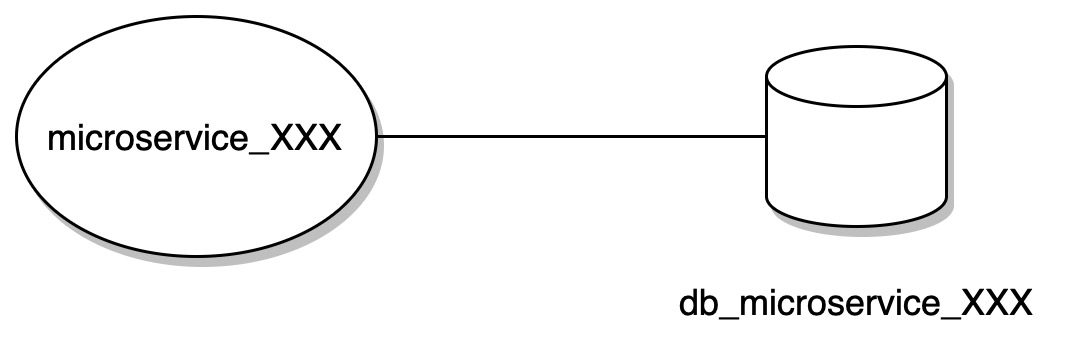
\includegraphics[width=\textwidth]{img/03-design/microservice-db.jpg}
    \caption{Un microservizio con il proprio database}
    \label{fig:microservice-db}
\end{figure}

A fronte di ciò sono stati identificati i seguenti microservizi:

\begin{itemize}
    \item \textbf{Notifications:} permette la gestione delle notifiche e lo status (online, ultimo accesso) degli utenti del sistema;

    \item \textbf{Users:} gestisce l'autenticazione degli utenti al sistema e tutti i dati relativi agli stessi. Inoltre, si occupa delle amicizie fra utenti;

    \item \textbf{Frontend:} fornisce l'accesso al sistema servendo la logica del client come Single Page Application;

    \item \textbf{Messages:} gestisce i messaggi degli utenti, sia nelle chat individuali, che per i canali testuali;

    \item \textbf{Monitoring:} permette il monitoraggio degli altri microservizi;

    \item \textbf{Piperchat:} gestisce la struttura di server e canali del sistema;

    \item \textbf{Webrtc:} gestisce tutto ciò che concerne \emph{WebRTC}, permettendo di istanziare video-chiamate all'interno del sistema.
\end{itemize}

%
%
%
\subsection{Comunicazione}

Al fine di permettere la comunicazione dei microservizi all'interno del sistema e permettere un'interazione con l'esterno, sono identificati i seguenti componenti:

\begin{itemize}
    \item \textbf{API Gateway:} componente che permette la comunicazione tra i client esterni al sistema, con i microservizi. Si occupa di redirezionare le richieste agli appositi servizi.

    \item \textbf{Broker:} componente che permette la comunicazione interna al sistema, fra i microservizi stessi.
\end{itemize}

\begin{figure}[htbp]
    \centering
    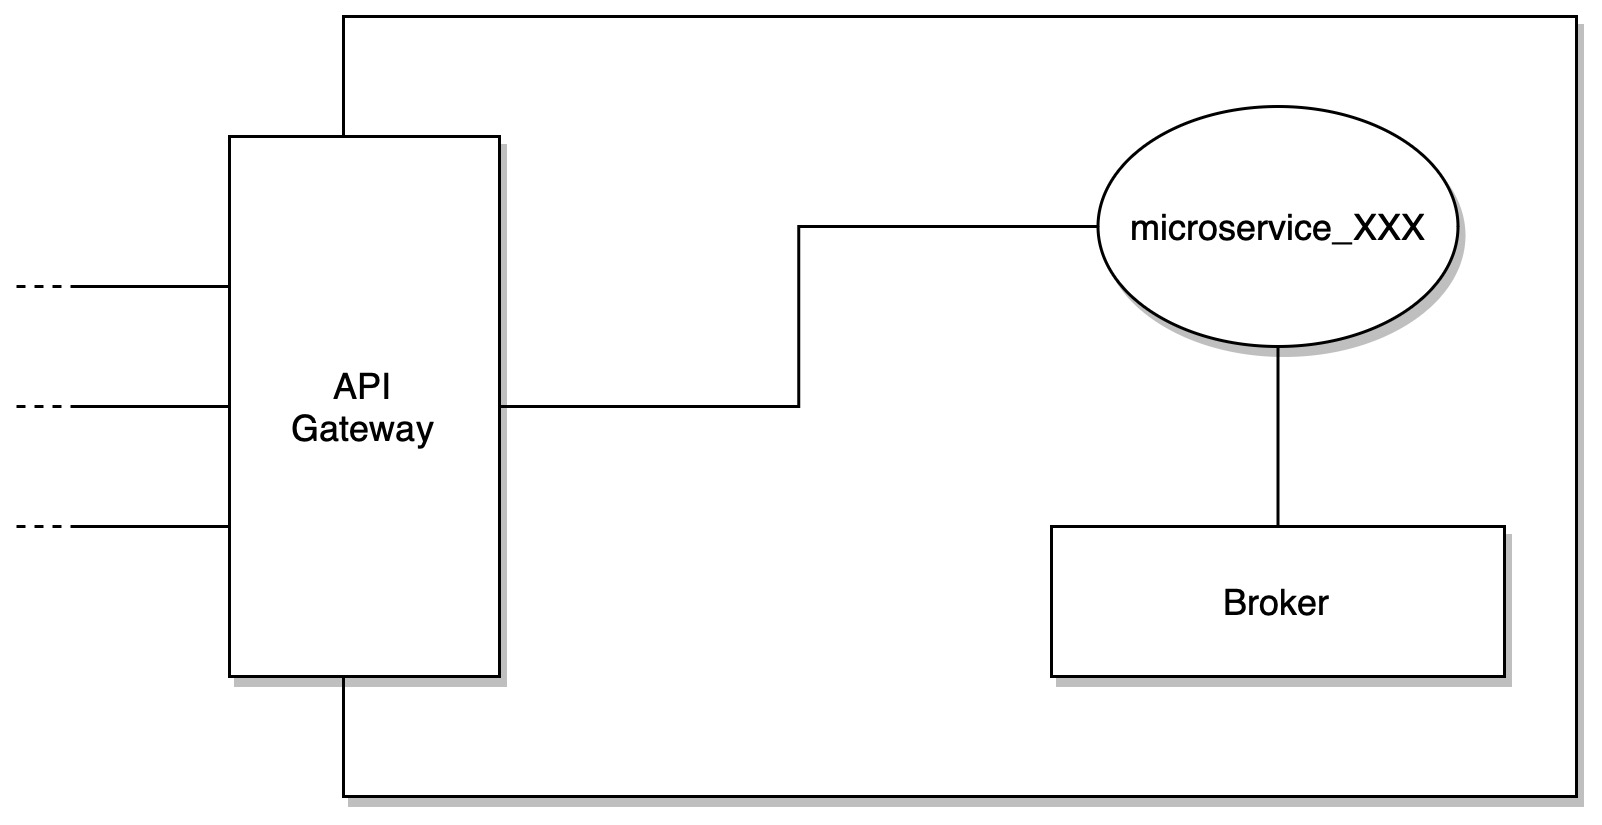
\includegraphics[width=\textwidth]{img/03-design/gateway-broker-microservice.jpg}
    \caption{Un microservizio collegato al Broker e all'API Gateway}
    \label{fig:gateway-broker-microservice}
\end{figure}

%
%
%
\subsection{L'architettura proposta}

Un utente, per accedere al servizio sfrutta l'\emph{API Gateway}.
In questo modo è possibile nascondere l'implementazione retrostante.

Di seguito è riportato lo schema architetturale del sistema.

\begin{figure}[htbp]
    \centering
    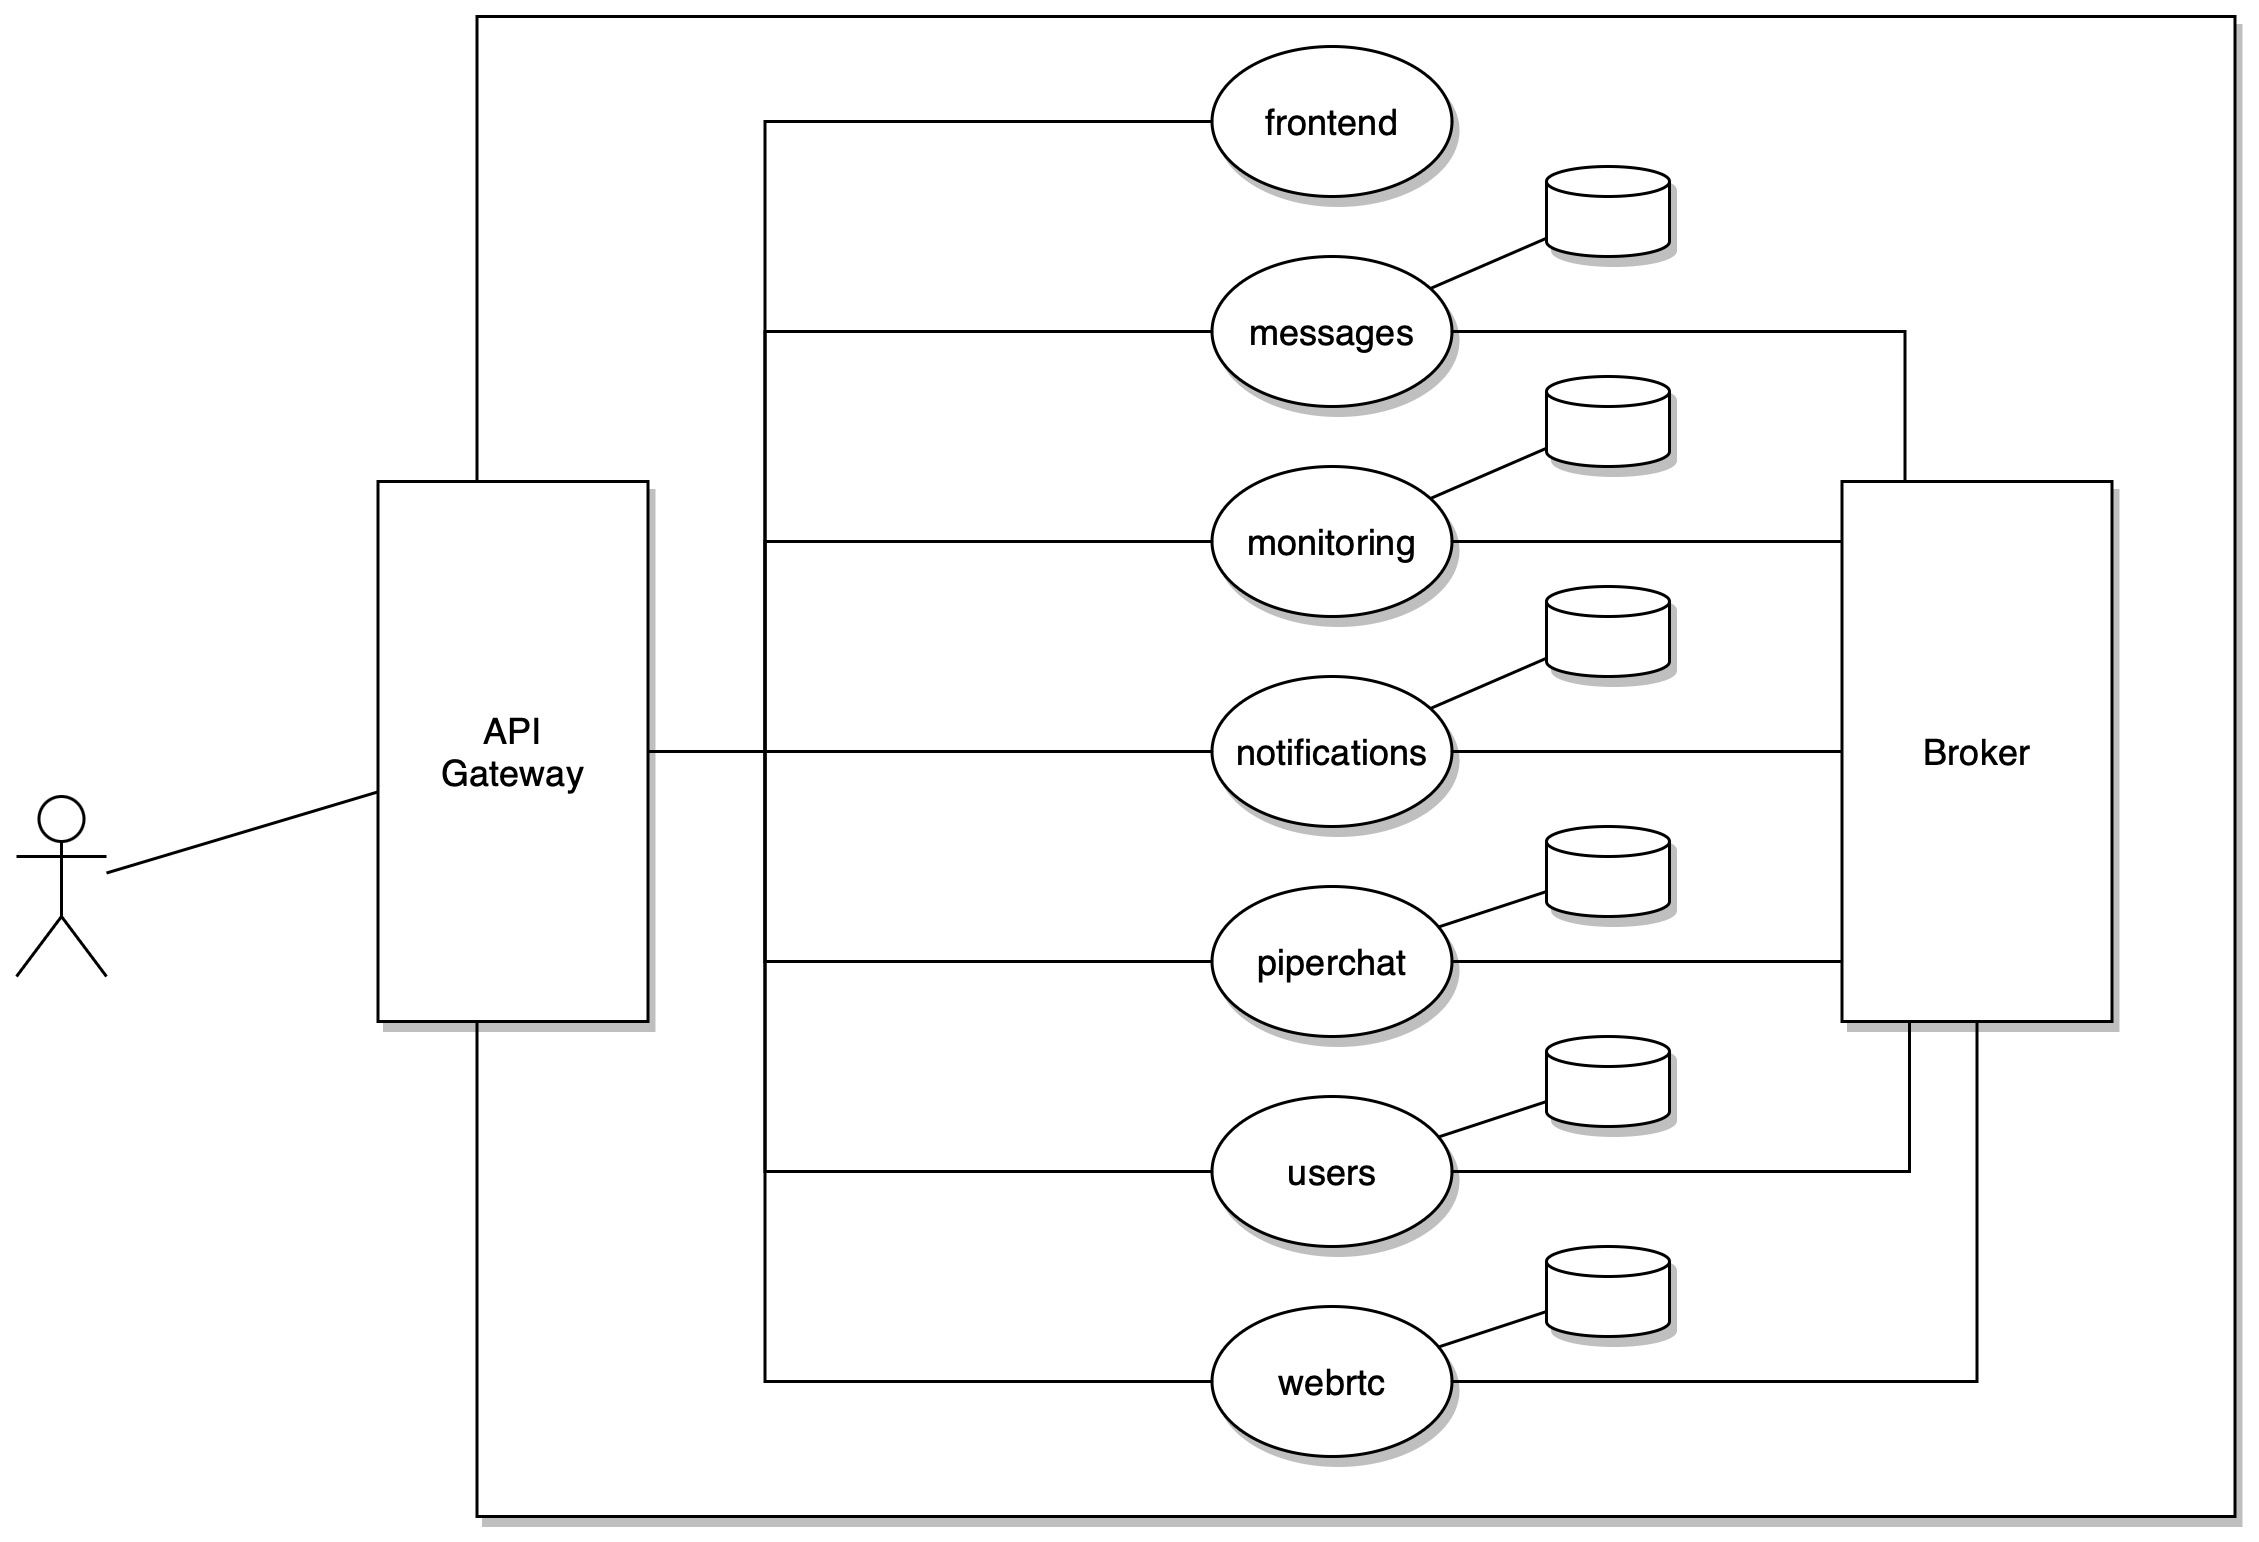
\includegraphics[angle=-90,width=0.95\textwidth]{img/03-design/architecture-schema.jpg}
    \caption{Architettura di Piperchat}
    \label{fig:piperchat-architecture}
\end{figure}


\chapter{Tecnologie}

%
%
%
\section{Stack MEVN}

L’applicazione è stata sviluppata sulla base dello stack MEVN, che come l’acronimo comprende le seguenti tecnologie:

\begin{itemize}
    \item \textbf{MongoDB}: È il database NoSQL utilizzato come backend per memorizzare i dati. MongoDB è flessibile, scalabile e adatto per la gestione di dati non strutturati o semistrutturati.

    \item \textbf{Express}: È un framework JavaScript per la creazione di server web. Express semplifica la gestione delle richieste HTTP, il routing e \\l'implementazione di middleware nel server.

    \item \textbf{Vue.js}: È un framework JavaScript progressivo per la creazione di interfacce utente. Vue.js è noto per la sua facilità d'uso e offre una solida architettura per lo sviluppo di interfacce utente interattive.

    \item \textbf{Node.js}:è un runtime per l'esecuzione di codice JavaScript.
\end{itemize}

%
%
%
\section{Strumenti, Framework \& Librerie utilizzati}
% Da riscrivere meglio

%
%
%
\subsection{Docker}

Docker è un software progettato per eseguire processi informatici in ambienti isolabili noti come \emph{container}, semplificando la creazione, la distribuzione e l'esecuzione di applicazioni.
%
I container includono il codice dell'applicazione, le librerie e le dipendenze, garantendo che l'applicazione funzioni in modo coerente su qualsiasi ambiente in cui venga eseguita.
%
Le principali caratteristiche di Docker includono:

\begin{enumerate}
    \item \textbf{Isolamento dell'ambiente}: Docker offre un alto grado di isolamento, consentendo alle applicazioni di essere eseguite indipendentemente senza interferire con altre applicazioni sullo stesso sistema.

    \item \textbf{Portabilità}: I contenitori Docker sono altamente portabili. Un contenitore Docker può essere eseguito su qualsiasi sistema che esegua Docker, indipendentemente dal sistema operativo sottostante.

    \item \textbf{Velocità e leggerezza}: I contenitori Docker sono avviati in pochi secondi e richiedono meno risorse rispetto alle macchine virtuali, rendendo Docker ideale per distribuzioni scalabili e veloci.
\end{enumerate}

%
%
%
\subsubsection{Utilizzo}

Docker è stato utilizzato per eseguire il deploy di tutti i componenti del sistema, tra cui:

\begin{itemize}
    \item Webserver per microservizi
    \item Database per microservizi
    \item Servizi di utility
    \item Broker
    \item API Gateway
\end{itemize}

%
%
%
\subsection{Swagger}

Swagger è un insieme di strumenti open source per progettare, creare, documentare e consumare servizi web RESTful, attraverso la specifica \emph{Open API}.
%
L'obiettivo principale di Swagger è semplificare e standardizzare il processo di sviluppo e integrazione di API, fornendo una documentazione interattiva e uno strumento per testare direttamente le API.

Le caratteristiche chiave di Swagger includono:

\begin{itemize}
    \item Definizione della API: Swagger utilizza il formato YAML o JSON per definire la struttura e i dettagli di un'API RESTful, specificando risorse, operazioni, parametri, tipi di dati, e altro ancora.
    
    \item Interfaccia Utente Interattiva: Genera automaticamente un'interfaccia utente interattiva (Swagger UI) basata sulla definizione dell'API. Questa interfaccia consente agli sviluppatori di esplorare e testare le API direttamente dal browser.

    \item Standardizzazione e Conformità: Swagger promuove la standardizzazione nelle API RESTful, migliorando la coerenza e la comprensione tra sviluppatori e team di sviluppo
\end{itemize}

\subsubsection{Utilizzo}

Con Swagger, è stato possibile creare documentazione dettagliata delle API, specificando dettagli come gli endpoint, i parametri, i tipi di dati, le risposte possibili e persino esempi di richieste e risposte.

La documentazione delle API del progetto è consultabile sulle Github Pages:
\url{https://zucchero-sintattico.github.io/piperchat/api/rest/}

%
%
%
\subsection{AsyncApi}

AsyncAPI è uno standard di specifica per la progettazione di API asincrone.
%
Simile a come OpenAPI è utilizzato per definire e documentare API sincrone, AsyncAPI è progettato specificamente per gestire le comunicazioni asincrone, come quelle basate su messaggi o eventi.

Le principali caratteristiche di AsyncAPI includono:

\begin{itemize}
    \item Comunicazioni Asincrone: AsyncAPI è progettato per modellare API che coinvolgono comunicazioni asincrone, dove la richiesta e la risposta non sono sincronizzate nel tempo.

    \item Documentazione Dettagliata: Come OpenAPI per API sincrone, AsyncAPI fornisce una specifica dettagliata per documentare aspetti come endpoint, messaggi, schemi dei dati, protocolli di trasporto e altri dettagli relativi alla comunicazione asincrona.

    \item Supporto per Protocolli Comuni: AsyncAPI supporta una varietà di protocolli comuni per la comunicazione asincrona, come MQTT, AMQP e WebSocket. Ciò consente una flessibilità nella progettazione delle API a seconda delle esigenze specifiche del progetto.
\end{itemize}

%
%
%
\subsubsection{Utilizzo}

AsyncAPI è stato utilizzato come strumento di supporto e di documentazione di tutte le tipologie di messaggi rappresentanti gli eventi che vengono scambiati tramite il broker all'interno dell'architettura a microservizi.

La documentazione delle API per i messaggi infra-servizi è consultabile sulle Github Pages:
\url{https://zucchero-sintattico.github.io/piperchat/api/infra-service/}

Inoltre, la tecnologia è stata sfruttata anche per la documentazione dei messaggi inviati ai client come notifiche di eventi.
Tale documentazione è disponibile al seguente link:
\url{https://zucchero-sintattico.github.io/piperchat/api/notification/}

%
%
%
\subsection{Traefik}

Traefik è un moderno \emph{reverse proxy} e \emph{load balancer} progettato per gestire il traffico web in ambienti complessi e distribuiti.
%
La sua funzione principale è quella di agire come un \emph{API Gateway}, instradando e distribuendo il traffico tra il frontend e i diversi microservizi del backend.

%
%
%
\subsubsection{Utilizzo}

Nel contesto del nostro progetto, l'utilizzo di Traefik è stato implementato in modo agevole e efficiente.
%
All'interno di ciascun file \emph{Docker Compose} relativo ai singoli servizi, abbiamo semplicemente specificato le richieste o le rotte accettate dal microservizio attraverso l'aggiunta di una label.
%
Questo approccio ci ha permesso di configurare facilmente e in modo dettagliato le direttive per il routing del traffico verso ciascun servizio, consentendo a Traefik di instradare le richieste in base alle specifiche esigenze di ciascun microservizio.

Di seguito è riportato un esempio della definizione delle rotte.

\begin{verbatim}
    labels:
      - |
        traefik.http.routers.users-service.rule=
        (Method(`GET`) && Path(`/friends`)) ||
        (Method(`GET`) && Path(`/whoami`)) ...
\end{verbatim}

%
%
%
\subsection{WebRTC}

\emph{WebRTC}, acronimo di "Web Real-Time Communication," è una tecnologia open-source che consente la comunicazione audio e video in tempo reale direttamente tra browser web senza richiedere plugin o software aggiuntivi.
%
È utilizzato per creare applicazioni di videoconferenza, chat video, streaming multimediale e altro.

Le principali caratteristiche di WebRTC includono:

\begin{enumerate}
    \item \textbf{Comunicazione peer-to-peer}: WebRTC consente ai browser di comunicare direttamente tra loro, evitando la necessità di server intermediari per la trasmissione di dati in tempo reale.

    \item \textbf{Supporto per audio e video}: WebRTC supporta la comunicazione audio e video in tempo reale, consentendo agli utenti di interagire tramite chat video o conferenze online.

    \item \textbf{Accesso ai dispositivi}: WebRTC consente l'accesso ai dispositivi hardware come telecamere e microfoni per abilitare la cattura audio e video.
\end{enumerate}

%
%
%
\subsubsection{Utilizzo}

Webrtc è stato utilizzato per la gestione delle video chiamate dei canali multimediali e infra-utente.
%
Questo ha permesso di evitare lo sviluppo di un servizio adibito allo streaming audio e video degli utenti, lasciando tale compito agli utenti stessi in maniera peer-to-peer.

%
%
%
\subsubsection{Funzionamento}

Nel contesto di WebRTC, ci sono tre concetti chiave: \textbf{offer}, \textbf{answer}, e \textbf{ICE candidates}.

\begin{itemize}
    \item \textbf{Offer}:
    L'offerta è il punto di partenza per l'inizializzazione di una connessione WebRTC.

    Un peer (la parte che inizia la connessione) crea un'offerta che specifica le sue preferenze per la sessione di comunicazione, inclusi i codec supportati, i parametri di sicurezza, etc.
    L'offerta è creata utilizzando l'API \textit{createOffer().}

    \item \textbf{Answer}:
    L'answer è generata dal peer destinatario in risposta all'offerta ricevuta.
    
    Il peer destinatario, dopo aver ricevuto l'offerta, crea una risposta che riflette le sue preferenze per la comunicazione.
    L'answer è creata utilizzando l'API \textit{createAnswer().}

    \item \textbf{ICE Candidates}:
    ICE (Interactive Connectivity Establishment) è un protocollo utilizzato per stabilire una connessione in presenza di reti complesse, come dietro firewall o NAT.
    I candidati ICE sono gli indirizzi IP e le porte su cui un peer può essere contattato.
    Durante il processo di offerta e risposta, i peer scambiano i loro candidati ICE utilizzando l'API onicecandidate.
    Il processo di raccolta dei candidati ICE è noto come "ICE gathering".
\end{itemize}

In sintesi, il flusso tipico di inizializzazione di una connessione WebRTC coinvolge la creazione di un'offerta da parte del peer iniziatore, la trasmissione di questa offerta al peer destinatario, la creazione di una risposta da parte del peer destinatario e, infine, lo scambio di candidati ICE per stabilire una connessione diretta tra i due peer.
%
Questo processo è fondamentale per consentire la comunicazione bidirezionale in tempo reale tra browser senza passare attraverso un server intermedio.

%
%
%
\subsubsection{Protocollo per videochiamate basato su eventi}

Per la gestione dello scambio di informazioni necessarie ad instaurare una comunicazione webrtc tra utenti è stato sviluppato un apposito servizio che opera su un protocollo che ha permesso di mettere in contatto tutti i partecipanti di una determinata sessione, in modo da avere un accesso uniforme e un aggiornamento reattivo all'arrivo o all'uscita degli utenti.

\begin{figure}[htbp]
    \centering
    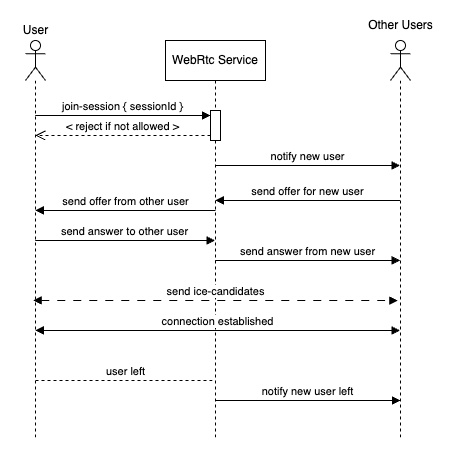
\includegraphics[width=\textwidth]{img/piperchat-WebRTC.drawio.png}
    \caption{Protocollo chiamate webrtc}
    \label{fig:webrtc-protocol}
\end{figure}

%
%
%
\subsection{SocketIO}

Socket.IO è una libreria JavaScript che fornisce una comunicazione bidirezionale in tempo reale tra il server e il client in applicazioni web.
%
È spesso utilizzata per implementare funzionalità di chat, giochi multiplayer, aggiornamenti in tempo reale e altre applicazioni che richiedono una comunicazione immediata tra il server e il browser.
%
Le principali caratteristiche di Socket.IO includono:

\begin{enumerate}
    \item \textbf{Comunicazione in tempo reale}: Socket.IO consente una comunicazione bidirezionale in tempo reale, consentendo agli utenti di ricevere aggiornamenti istantanei dal server.

    \item \textbf{Supporto multipiattaforma}: Socket.IO è compatibile con diverse piattaforme e browser, consentendo una comunicazione uniforme su molteplici dispositivi.

    \item \textbf{Messaggi personalizzati}: Gli sviluppatori possono definire messaggi personalizzati per gestire eventi specifici nell'applicazione, come messaggi di chat o aggiornamenti di gioco.

    \item \textbf{Riconnessione automatica}: Socket.IO supporta la riconnessione automatica in caso di perdita di connessione, garantendo che gli utenti rimangano connessi.

    \item \textbf{Ampia adozione}: Socket.IO è ampiamente utilizzato nella comunità di sviluppatori ed è supportato da molte piattaforme e framework.

\end{enumerate}

%
%
%
\subsubsection{Utilizzo}

Socket.io è stato utilizzato per sviluppare i sistemi di comunicazione con i microservizi che richiedevano un aggiornamento continuo di informazioni o uno scambio di dati reciproco.

In particolare è stato implementato nei seguenti sistemi:

\begin{itemize}
    \item Sistema di notifiche: poiché era necessaria un elevata reattività e una continua connessione al server da parte degli utenti per ricevere le notifiche.

    \item Gestione dello status online degli utenti.
    
    \item Sistema di videochiamate: sfruttato per la gestione del protocollo per l'accesso a videochiamate e per tutti gli aggiornamenti che ne conseguono come join e left di un utente.
\end{itemize}

%
%
%
\subsection{Quasar}

Quasar Framework è un framework open-source basato su Vue.js, progettato per semplificare lo sviluppo di applicazioni web e mobile con un unico codice sorgente.
%
È noto per la sua flessibilità e la capacità di generare applicazioni per diverse piattaforme.
%
Le caratteristiche principali di Quasar Framework includono:

\begin{enumerate}
    \item \textbf{Componenti Vue.js predefiniti}: Quasar offre una vasta libreria di componenti Vue.js personalizzati e ricchi di funzionalità, che semplificano la creazione di interfacce utente sofisticate.

    \item \textbf{Responsive Design}: Le applicazioni Quasar possono essere facilmente rese responsive per adattarsi a diversi dispositivi e dimensioni dello schermo.

    \item \textbf{Material Design}: Quasar aderisce a Material Design di Google, offrendo un aspetto moderno e uniforme per le applicazioni.
\end{enumerate}

%
%
%
\subsubsection{Utilizzo}

Quasar è stato impiegato per i componenti principali dell'interfaccia utente che il framework offre.

%
%
%
\subsection{Pinia}

Pinia JS è una libreria di gestione dello stato progettata per applicazioni Vue.js.
%
Essa fornisce un'architettura di gestione dello stato centralizzata e reattiva, offrendo uno store centralizzato per memorizzare e gestire lo stato dell'applicazione.
%
Pinia si basa sui concetti principali di Vue.js, come la reattività e la gestione delle modifiche dello stato in modo efficiente.
%
Questo strumento consente agli sviluppatori di scrivere codice pulito e manutenibile, facilitando la gestione dello stato dell'applicazione Vue.js.

%
%
%
\subsubsection{Utilizzo}

Nella nostra applicazione Vue, lo stato globale è stato gestito tramite la definizione di svariati store.
%
Ogni store è stato progettato per occuparsi di specifici aspetti funzionali dell'applicazione, fornendo una struttura chiara e distintiva per la gestione dei dati.

Sono stati definiti i seguenti store:

\begin{itemize}
    \item \textbf{Store `app':} Gestisce le informazioni globali dell'applicazione.
    
    \item \textbf{Store `friend':} Si occupa della gestione delle informazioni relative agli amici all'interno dell'applicazione.
    
    \item \textbf{Store `messages':} Gestisce la logica e i dati relativi ai messaggi.

    \item \textbf{Store `photo':} Gestisce il salvataggio e la fruizione delle foto all'interno dell'applicazione, in particolare è stato usato per fare caching delle foto degli utenti.

    \item \textbf{Store `users-status':} Gestisce le informazioni relativo allo stato degli utenti (online/offile/ultimo accesso) tramite un sistema di caching che ne permette la fruizione in modo semplice.
    
    \item \textbf{Store `monitoring':} Si occupa della raccolta e visualizzazione dei dati relativi al monitoraggio dei microservizi dell'applicazione.
    
    \item \textbf{Store `notifications':} Gestisce le notifiche dell'applicazione, inclusi avvisi, notifiche push e loro gestione.
    
    \item \textbf{Store `server':} Gestisce le comunicazioni relative ai server e ai canali.
    
    \item \textbf{Store `user':} Si occupa delle informazioni e delle azioni relative all'utente, inclusi i dati del profilo e le operazioni di autenticazione.
    
    \item \textbf{Store `webrtc':} Gestisce le funzionalità e lo stato relativi alle comunicazioni in tempo reale tramite WebRTC, inclusi audio, video e connettività.
\end{itemize}

%
%
%
\section{Linguaggi}

I linguaggi di programmazione utilizzati all'interno del progetto sono i seguenti:

\begin{itemize}
    \item \textbf{Typescript}: sia per il backend che per il frontend

    \item \textbf{HTML}: per la realizzazione delle web pages

    \item \textbf{CSS}: per i fogli di stile 
\end{itemize}


\chapter{Codice}

\section{Definizione API}

Per quanto riguarda la gestione delle api dei vari microservizi si è optato per avere una struttura che rappresentasse ogni endpoint, incapsulando sia i dati richiesti sia le possibili risposte.

A supporto di ciò è stato creato un modulo \textbf{api} che incapsula tutti gli endpoint del backend con le relativi informazioni.

Tale modulo viene sfruttato sia dal backend, per avere un typing migliore e un controllo di validazione dei parametri richiesti, sia dal frontend per sapere già quali sono codice di risposta e tipologie di risposta per un determinato endpoint.

\begin{lstlisting}[style=typescript, caption={Definizione API}, label=lst:login:api]
export namespace LoginApi {
  export namespace Request {
    export type Body = {
      username: string
      password: string
    }
  }

  export namespace Responses {
    export class Success extends Response {
      statusCode = 200
      message = 'Logged in' as const
      jwt: string
    }
  }

  export namespace Errors {
    export class UsernameOrPasswordIncorrect extends ErrorResponse {
      statusCode = 401
      error = 'Username or password incorrect' as const
    }
  }
}
\end{lstlisting}

\section{Definizione Endpoint}

Una volta costruita la struttura rappresentante le singole API è stata creata l'utility \textbf{Route}, che a partire da un api permette di implementare l'endpoint aggiungendo il supporto automatico alla validazione dei dati in modo che se i dati in ingresso non sono corretti l'handler non venga triggherato e venga restituito un messaggio di errore \textit{Bad Request}.
%
Inoltre permette e di dichiarare come reagire per ogni tipo di errore senza doverli controllare all'interno dell'handler.

Altra utilità offerta dalla classe è il typing dei parametri della richiesta basati sulle api specificate.

\begin{lstlisting}[style=typescript, caption={Definizione API}, label=lst:login:route]
export const LoginApiRoute = new Route<
  ...
>({
  method: 'post',
  path: '/login',
  schema: LoginApi.Request.Schema,
  handler: async (req, res) => {
    const token = await authController.login(req.body.username, req.body.password)
    res.sendResponse(new LoginApi.Responses.Success(token))
  },
  exceptions: [
    {
      exception: InvalidUsernameOrPassword,
      onException: (e, req, res) => {
        res.sendResponse(new UsernameOrPasswordIncorrect())
      },
    },
  ],
})
\end{lstlisting}

\section{Definizione dei Controller}

Per interfacciarsi con gli endpoint del backend sono quindi stati scritti i \textbf{Controller} lato frontend, che incapsulano la gestione delle API e sfruttano il modulo \textit{api} per ottenere un typing delle richieste e delle risposte.

\begin{lstlisting}[style=typescript, caption={Definizione Controller}, label=lst:controller]
export class AuthControllerImpl extends AxiosController implements AuthController {
  async register(request: RegisterApi.Request.Type): Promise<RegisterApi.Response> {
    const body = request as RegisterApi.Request.Body
    return await this.post<RegisterApi.Response>('/auth/register', body)
  }

  async login(request: LoginApi.Request.Type): Promise<LoginApi.Response> {
    const body = request as LoginApi.Request.Body
    return await this.post<LoginApi.Response>('/auth/login', body)
  }

  async logout(): Promise<LogoutApi.Response> {
    return await this.post<LogoutApi.Response>('/auth/logout', {})
  }

  async refreshToken(): Promise<RefreshTokenApi.Response> {
    return await this.post<RefreshTokenApi.Response>(
        '/auth/refresh-token', {})
  }
}
\end{lstlisting}

%
%
%
\section{Definizione degli Store}

Come già accennato in  precedenza, lo stato globale dell'applicazione è stato gestito tramite gli store di Pinia.
%
Di seguito un esempio dell'utilizzo per implementare il caching delle foto degli utenti:

\begin{lstlisting}[style=typescript, caption={Definizione di uno Store}, label=lst:store]
export const usePhotoStore = defineStore('photo', () => {
  const userController: UserController = new UserControllerImpl()
  const usersPhotos = ref<Record<string, string | undefined>>({})

  async function reloadUserPhoto(targetUsername: string) {
    try {
      const response = await userController.getUserPhoto({
        username: targetUsername
      })
      if (response.statusCode === 200) {
        const typed = response as GetUserPhotoApi.Responses.Success
        if (typed.photo.data !== undefined) {
          usersPhotos.value[targetUsername] =
            'data:image/jpeg;base64,' +
            btoa(
              new Uint8Array((typed.photo.data as any).data).reduce(
                (data, byte) => data + String.fromCharCode(byte),
                ''
              )
            )
        }
      }
    } catch (e) {
      console.log(e)
    }
  }

  function getUserPhoto(targetUsername: string): Ref<string | undefined> {
    if (usersPhotos.value[targetUsername] === undefined) {
      reloadUserPhoto(targetUsername)
    }
    return computed(() => usersPhotos.value[targetUsername])
  }

  return {
    reloadUserPhoto,
    getUserPhoto
  }
})

\end{lstlisting}

%
%
%
\section{Definizione di Componenti}

Nella sviluppo della nostra applicazione, abbiamo adottato un approccio modulare, suddividendola in diversi componenti che sono stati sviluppati utilizzando le \textit{Composition API} offerte da Vue.
%
Per migliorare l'estetica e lo stile di quest'ultimi, abbiamo arricchito ogni componente sfruttando le funzionalità offerte dal framework \textit{Quasar}:

\begin{lstlisting}[style=typescript, caption={Definizione Components}, label=lst:component]
<script setup lang="ts">
import { onMounted } from 'vue'
import AreaHeader from './AreaHeader.vue'
import EmptyContent from './EmptyContent.vue'
import ChatArea from './chat/ChatArea.vue'
import WebrtcArea from './video/WebrtcArea.vue'
import { useAppStore } from '@/stores/app'

const appStore = useAppStore()
</script>

<template>
  <q-page class="q-pa-auto">
    <q-layout view="lHh Lpr lFf" container style="min-height: inherit">
      <AreaHeader />
      <EmptyContent v-if="!appStore.isMessageSection && !appStore.isVideoSection" />
      <ChatArea v-if="appStore.isMessageSection" />
      <WebrtcArea v-if="appStore.isVideoSection" />
    </q-layout>
  </q-page>
</template>
\end{lstlisting}


\chapter{Test}

%
%
%
\section{Jest}

Ogni microservizio definisce degli \emph{Unit Testing} mediante \emph{Jest} in modo da verificare la correttezza delle richieste e delle relative risposte, dei singoli microservizi.

In questo modo, siamo stati in grado di concentrarci sui seguenti aspetti durante i test:

\begin{itemize}
    \item Verifica della correttezza delle richieste fornite.

    \item Verifica della correttezza delle risposte fornite da diverse richieste.

    \item Test di integrazione per garantire che i vari endpoint si comportino correttamente, potendo verificare i side effect di una richiesta, eseguendo richieste successive.
\end{itemize}

Questo approccio ci ha permesso di sviluppare test solidi e garantire che i microservizi rispettassero gli standard richiesti.

%
%
%
\section{Microservizi}

Tutti i microservizi posseggono una suite di test.
%
Di seguito un esempio con il core del testing del servizio degli utenti:

\begin{lstlisting}[style=typescript, caption={microservice Test}, label=lst:login:route:test]
const userMicroservice: Microservice = new Microservice(UserServiceConfiguration)
let request: supertest.SuperTest<supertest.Test>

beforeAll(async () => {
  await userMicroservice.start()
  request = supertest(userMicroservice.getServer())
})

afterAll(async () => {
  await userMicroservice.stop()
})

afterEach(async () => {
  await userMicroservice.clearDatabase()
})

describe('Register', () => {
  it('A user must provide username, password and email', async () => {
    let response = await request
      .post('/auth/register')
      .send({ username: 'test', password: 'test' })
    expect(response.status).toBe(400)
    // other test stuff
    response = await request
      .post('/auth/register')
      .send({ username: 'test', password: 'test', email: 'test' })
    expect(response.status).toBe(200)
  })
    // other test stuff
})

describe('Login', () => {
    it('A user should provide username and password to login', async () => {
        let response = await register('test', 'test', 'test')
        response = await request.post('/auth/login').send({ username: 'test' })
        expect(response.status).toBe(400)
        response = await request.post('/auth/login').send({ password: 'test' })
        expect(response.status).toBe(400)
        response = await request
          .post('/auth/login')
          .send({ username: 'test', password: 'test' })
        expect(response.status).toBe(200)
    })
    // other test stuff
})

describe('Logout', () => {
  it('A user should be able to logout', async () => {
    let response = await createUserAndLogin('test', 'test', 'test')
    const cookie = response.header['set-cookie']
    response = await request.post('/auth/logout').set('Cookie', cookie)
    expect(response.status).toBe(200)
  })
    // other test stuff
})

describe('Refresh token', () => {
  it('A user should be able to refresh token', async () => {
    let response = await createUserAndLogin('test', 'test', 'test')
    const cookie = response.header['set-cookie']
    response = await request.post('/auth/refresh-token').set('Cookie', cookie)
    expect(response.status).toBe(200)
    expect(response.header['set-cookie']).toHaveLength(1)
  })
    // other test stuff
})

\end{lstlisting}

%
%
%
\section{Utenti}

Il sito è stato messo a disposizione di diversi gruppi di utenti per valutarne l'utilizzo e raccogliere feedback.
%
Questa fase di test è stata cruciale per valutare la facilità d'uso e comprendere come migliorare l'esperienza complessiva degli utenti.
%
Dopo l'utilizzo, è stato chiesto loro di compilare un Google Form, consentendo di raccogliere opinioni e osservazioni dirette.

Attraverso questo processo, siamo stati in grado di individuare aree che richiedono miglioramenti e identificare possibili bug che non erano emersi durante lo sviluppo iniziale.
%
I feedback degli utenti hanno fornito preziose informazioni su aspetti che possono essere ottimizzati per garantire un'esperienza più fluida e soddisfacente.

\begin{figure}[htbp]
    \centering
    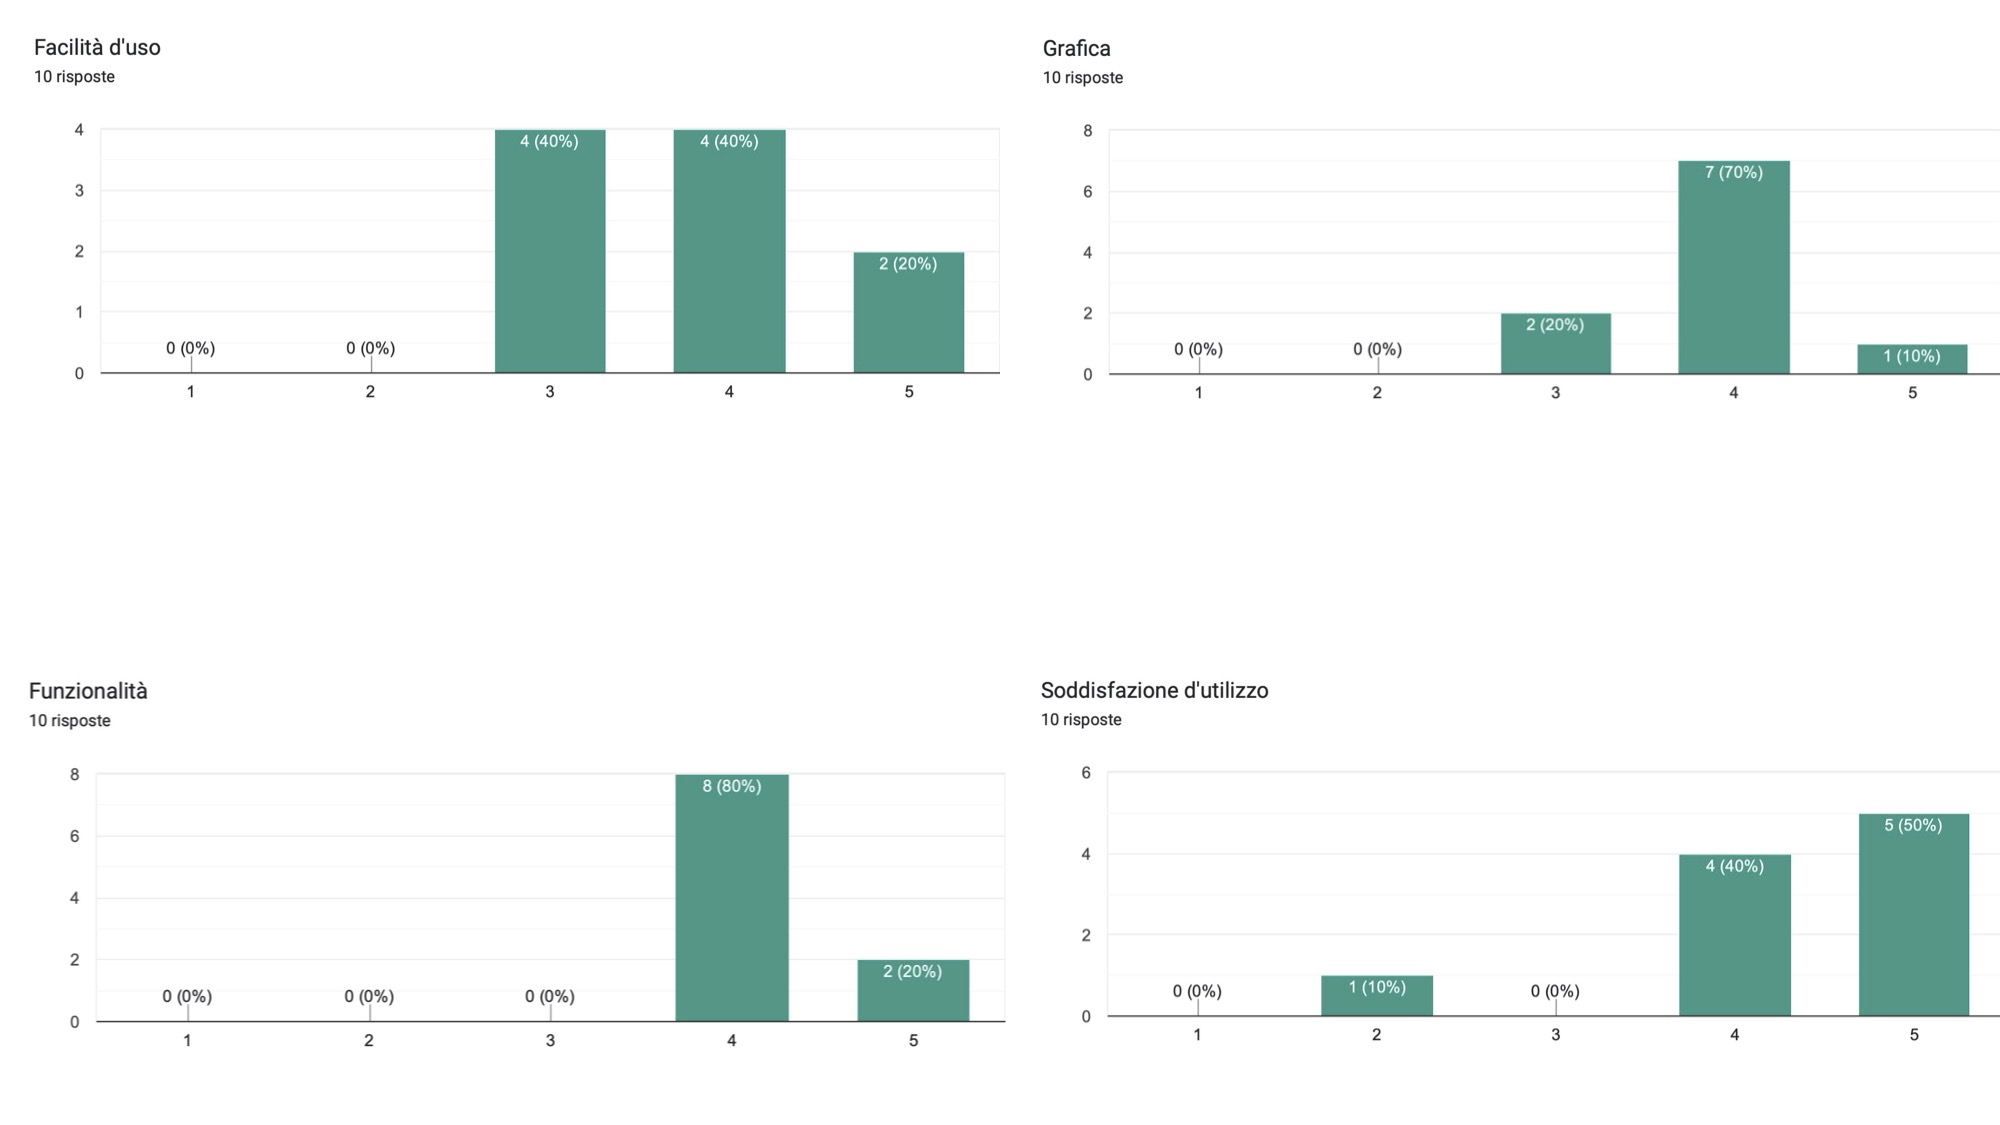
\includegraphics[width=\textwidth]{img/GraficiUtenti.jpg}
    \caption{Grafici del questionario rivolto agli utenti}
    \label{fig:grafico_user_expirience}
\end{figure}

\textbf{Grafica:}
    Abbiamo ricevuto una valutazione media di 3,8 su 5 per l'aspetto visivo del nostro prodotto. Le valutazioni variano da 3 a 5. La maggior parte degli utenti sembra apprezzare l'aspetto visuale, sebbene alcuni suggeriscano possibili miglioramenti.

\textbf{Facilità d'uso:}
    L'usabilità ha ottenuto una valutazione media di 3,5 su 5, con valutazioni comprese tra 3 e 5. Alcuni utenti potrebbero aver riscontrato difficoltà nell'utilizzo del sistema, indicando la necessità di miglioramenti per rendere il sistema più accessibile.
    
\textbf{Funzionalità:}
    Abbiamo ottenuto una valutazione media di 4,1 su 5 per le funzionalità offerte. La maggior parte degli utenti sembra apprezzare le funzionalità del nostro sistema, anche se ci sono alcune valutazioni più basse che indicano un gruppo di utenti che sente la necessità di un' esperienza più ampia.
    
\textbf{Soddisfazione d'utilizzo:}
    La soddisfazione media è di 4,3 su 5. La maggior parte degli utenti sembra essere soddisfatta dell'esperienza complessiva, tuttavia vi sono alcune valutazioni più basse che potrebbero indicare potenziali aree di miglioramento.

In generale, i punteggi più elevati sono stati attribuiti alla `Soddisfazione d'utilizzo' e alle `Funzionalità', mentre la `Grafica' e la `Facilità d'uso' presentano valutazioni più variabili.
%
Questi risultati ci offrono un'idea del livello di apprezzamento per il nostro prodotto e allo stesso tempo ci indicano dove concentrare gli sforzi per migliorare, specialmente riguardo all'usabilità e all'aspetto visivo, al fine di offrire un'esperienza più coerente e soddisfacente per tutti gli utenti.

%
%
%
\section{Accessibilità}

Per testare i requisiti di accessibilità abbiamo utilizzato lo strumento integrato in Safari, il quale analizzando l'applicazione ci ha fornito il seguente feedback:

\begin{figure}[H]
    \centering
    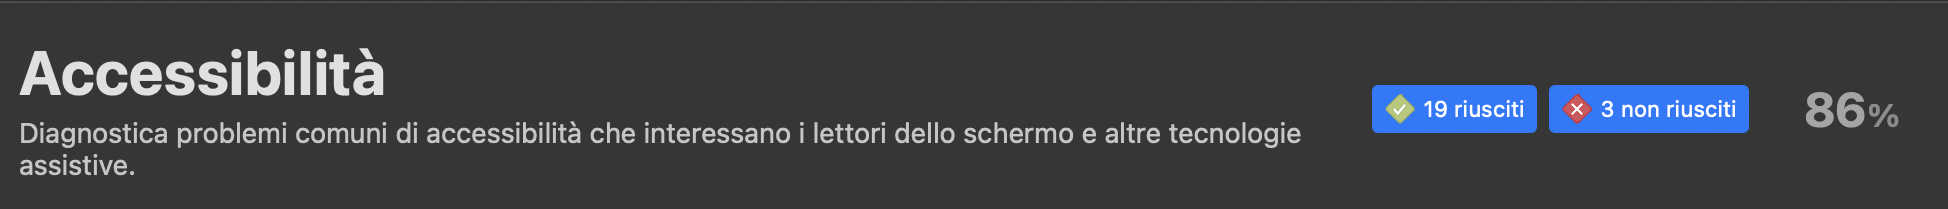
\includegraphics[width=1\textwidth]{img/accessibility.png}
    \caption{Test d'accessibilità di Safari}
    \label{fig:mockup-accessibility}
\end{figure}

Come possiamo notare non tutti i test hanno riscontrato un feedback positivo, tuttavia, alcuni di questi dipendono da Quasar, ovvero il framework utilizzato per lo sviluppo dei componenti, in relazione a ciò abbiamo dovuto trovare dei compromessi.
%
L'impiego di layout innestati ha generato dei conflitti che si sono rivelati piuttosto complessi da risolvere.
%
La combinazione di questi layout ha causato problemi che, purtroppo, non sono stati facilmente gestibili a causa delle restrizioni intrinseche del framework.
%
Abbiamo cercato soluzioni alternative, ma gli ostacoli persistenti hanno richiesto più tempo del previsto per essere affrontati in modo efficace.


\chapter{Deployment}

L'applicazione è strutturata mediante i seguenti container:

\begin{itemize}
    \item Frontend Service: container che serve il Frontend sotto forma di Single Page Application.

    \item Messages Service e relativo Db: servizio responsabile della gestione dei messaggi testuali dell'applicazione (invio, ricezione, ecc...).

    \item Monitoring Service e relativo Db: servizio responsabile del monitoraggio dello stato di tutti i microservizi.

    \item Notifications Service e relativo Db: servizio responsabile delle notifiche degli utenti. Inoltre, detiene l'online status degli utenti del sistema.

    \item Piperchat Service e relativo Db: servizio responsabile della gestione dei Server e dei Canali dell'applicazione (creazione, modifica, partecipanti, ecc...).

    \item Users Service e relativo Db: servizio responsabile della gestione degli utenti dell'applicazione (login, registrazione, amicizie, ecc...).

    \item WebRTC Service e relativo Db: servizio responsabile della gestione delle chiamate infra-utenti e dei canali multimediali.

    \item Broker: container che ospita un server di \emph{RabbitMQ} per permettere lo scambio di messaggi all'interno del sistema

    \item Coturn: container che ospita il server \emph{TURN} (\url{https://github.com/coturn/coturn})

    \item Gateway: container che ospita l'\emph{API Gateway} realizzato con \emph{Traefik}. 

    \item Inspector: container di \emph{utility} per debuggare e/o ispezionare i servizi dall'interno della rete.
\end{itemize}

Per ogni microservizio quindi, viene effettuato il deploy di due diversi container, uno per il Webserver, mentre l'altro per il relativo database non relazionale.

Ogni microservizio possiede le seguenti reti docker:

\begin{itemize}
    \item Frontend: Per ricevere le richieste dal frontend tramite il Gateway.

    \item Backend: Per comunicare con gli altri microservizi (nel nostro caso tramite message broker).

    \item Microservicename-network: Rete interna del microservizio, utile alla comunicazione con il proprio database.
\end{itemize}

%
%
%
\section{Microservice deploy}

Per ogni microservizio è stato scritto un file \texttt{Docker Compose}.

Esempio di Docker compose relativo al singolo microservizio:

\begin{verbatim}
services:
  piperchat-service:
    image: piperchat
    command: [
        'npm', 
        'run', 
        '--workspace', 
        './services/piperchat', 
        'start'
    ]
    expose:
      - '${PIPERCHAT_SERVICE_PORT}'
    depends_on:
      db-piperchat-service:
        condition: service_healthy
      broker:
        condition: service_healthy
    networks:
      piperchat-network:
      backend:
        aliases:
          - ${PIPERCHAT_SERVICE_NAME}
      frontend:
    environment:
      - 'PORT=${PIPERCHAT_SERVICE_PORT}'
      - 'AMQP_URI=${BROKER_URI}'
      - 'MONGO_URI=
      mongodb://db-piperchat-service:27017/piperchat'
    labels:
      - |
        traefik.http.routers.piperchat-service.rule=
        (Method(`GET`, `POST`) 
            && Path(`/servers`)) ||
        (Method(`GET`, `PUT`, `DELETE`) 
            && Path(`/servers/{serverId:[^/]+}`)) ||
        (Method(`GET`, `POST`, `DELETE`) 
            && Path(`/servers/{serverId:[^/]+}/participants`)) ||
        (Method(`DELETE`) 
            && Path(`/servers/{serverId:[^/]+}/participants/{userId:[^/]+}`)) ||
        (Method(`GET`, `POST`) 
            && Path(`/servers/{serverId:[^/]+}/channels`)) ||
        (Method(`GET`, `PUT`, `DELETE`) 
            && Path(`/servers/{serverId:[^/]+}/channels/{channelId:[^/]+}`))

  db-piperchat-service:
    image: mongo
    expose:
      - '27017'
    volumes:
      - './.docker/db-piperchat:/data/db'
    healthcheck:
      test: |
        host=`hostname --ip-address || echo '127.0.0.1'`;
        mongo --quiet $${host}/test --eval 
        'quit(db.runCommand({ ping: 1 }).ok ? 0 : 2)' && echo 0 || echo 1
    networks:
      - piperchat-network

networks:
  piperchat-network:

\end{verbatim}

%
%
%
\section{Architecture deploy}

Avendo realizzato per ogni microservizio un apposito file  di \texttt{Docker Compose}, è stato utilizzato uno script bash per automatizzare l'unione di quest'ultimi ed eseguire il deploy dell'intera architettura.

Questo script si trova nella cartella root del progetto e si chiama \texttt{./deploy.sh}

Di seguito ne viene riportato un estratto:

\begin{verbatim}
docker compose \
    --project-name piperchat \
    --project-directory . \
    --env-file ./.env \
    -f ./services/broker/docker-compose.yaml \
    -f ./services/frontend/docker-compose.yaml \
    -f ./services/gateway/docker-compose.yaml \
    ...
    up
\end{verbatim}

\begin{figure}[htbp]
    \centering
    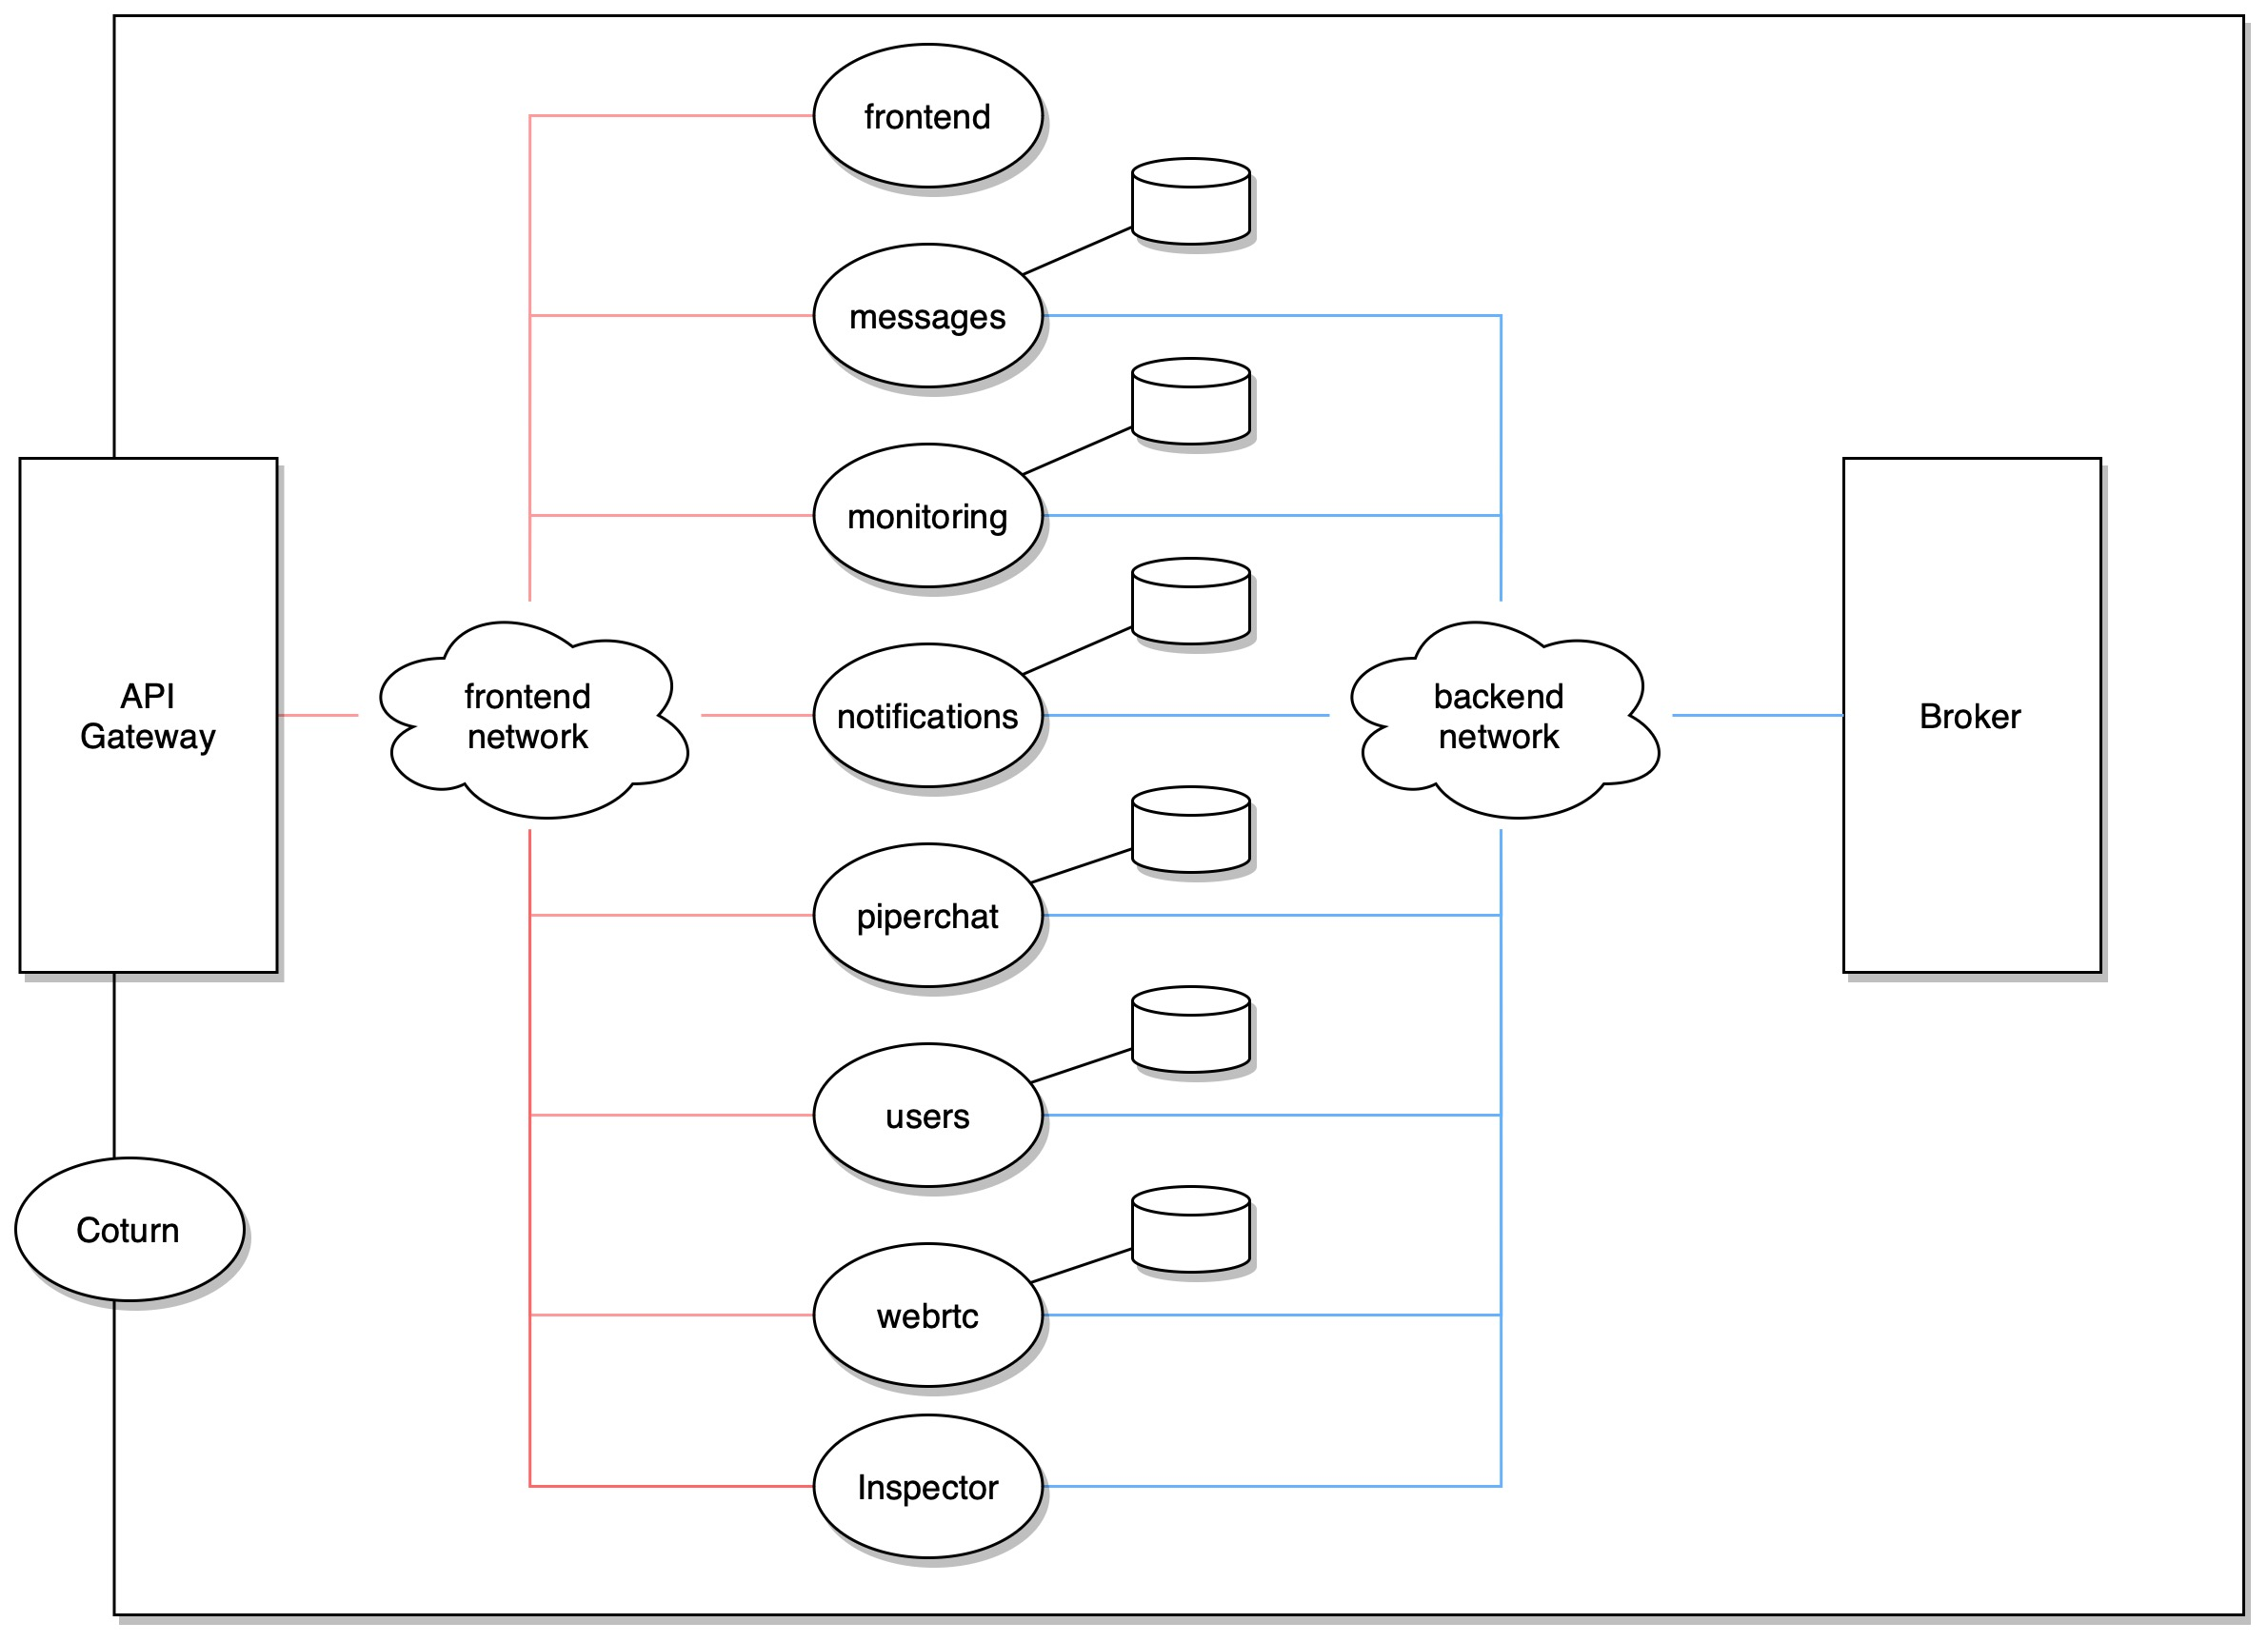
\includegraphics[width=0.85\textwidth]{img/07-deployment/architecture-deployment.jpg}
    \label{fig:architecture-deployment}
\end{figure}

%
%
%
\newpage
\section{Testing deploy}

Per effettuare il testing lato Backend, è stato realizzato un ulteriore \texttt{Docker Compose} il quale ci ha permesso deployare un infrastruttura "alleggerita", dotata unicamente dei container necessari a testare i singoli microservizi, nonché:

\begin{itemize}
    \item Un'istanza del Broker

    \item Un'istanza del database

    \item Un'istanza di Mongo Express per visualizzare il database
\end{itemize}

Questo \texttt{Docker Compose} è situato nella cartella \texttt{/dev}, insieme allo script che ne automatizza l'esecuzione, chiamato \texttt{runDev.sh}.

Di seguito riportato il \texttt{Docker Compose} dell'infrastruttura usata per il testing:

\begin{verbatim}
services:
  db-service:
    image: mongo
    ports:
      - '27017:27017'
    healthcheck:
      test: |
        host=`hostname --ip-address || echo '127.0.0.1'`;
        mongo --quiet $${host}/test --eval
            'quit(db.runCommand({ ping: 1 }).ok ? 0 : 2)' && echo 0 || echo 1

  broker:
    image: rabbitmq:3-management-alpine
    ports:
      - '5672:5672'
      - '15672:15672'
    healthcheck:
      test: ['CMD', 'rabbitmq-diagnostics', '-q', 'ping']

  mongo-express:
    image: mongo-express:latest
    restart: always
    ports:
      - '8081:8081'
    environment:
      ME_CONFIG_MONGODB_SERVER: 'db-service'
    depends_on:
      db-service:
        condition: service_healthy

\end{verbatim}


\section{Conclusioni}

Il progetto Piperchat è stato sviluppato con l'obiettivo di creare una piattaforma di comunicazione ispirata a Discord, offrendo agli utenti la possibilità di interagire in varie forme, creare connessioni sociali e gestire server personalizzati. L'architettura a microservizi è stata scelta per gestire la complessità del sistema, consentendo una maggiore coesione e scalabilità.

Durante lo sviluppo, sono stati affrontati diversi aspetti, tra cui la gestione delle amicizie, la messaggistica, la creazione e gestione di server e canali multimediali. L'implementazione di funzionalità come notifiche, chiamate vocali e video ha arricchito l'esperienza dell'utente.

La valutazione della qualità del software prodotto ha considerato aspetti cruciali come funzionalità, affidabilità, scalabilità, sicurezza, usabilità e prestazioni. L'approccio a microservizi ha dimostrato la sua efficacia nel garantire una struttura modulare e gestibile.

\subsection{Sviluppi futuri}
A causa delle scarse tempistiche, l'implementazione della dashboard relativa ai log dell'intera applicazione, è stata messa in secondo piano.
Detto ciò dunque, la prima feature da realizzare in termini di sviluppi futuri sarebbe proprio quest'ultima.

Altro miglioramento che potremmo apportare alla nostra applicazione, riguarderebbe il deploy dell'architettura, difatti attualmente, l'applicazione di videochat viene distribuita utilizzando Docker Compose con un approccio basato su una singola macchina. Tuttavia, per migliorare la scalabilità, la resilienza e la gestione delle risorse, è previsto un futuro passaggio a un'architettura basata su Docker Swarm.


\subsection{Cosa abbiamo imparato}

Durante lo sviluppo di Piperchat, abbiamo acquisito una comprensione approfondita dell'architettura a microservizi e delle sfide associate. Abbiamo imparato a bilanciare aspetti cruciali come la sicurezza, la scalabilità e l'usabilità in un progetto di comunicazione in tempo reale.

La collaborazione tra diversi team per lo sviluppo dei singoli microservizi e la gestione di comunicazione tra di essi attraverso un message broker hanno ampliato la nostra conoscenza delle best practice nello sviluppo di sistemi distribuiti.

Inoltre, l'importanza di valutare la qualità del software in termini di funzionalità, affidabilità e prestazioni ci ha fornito un quadro completo delle sfide e delle opportunità nell'implementazione di una piattaforma di comunicazione complessa come Piperchat.


% \bibliographystyle{plain}
% \bibliography{references}
\end{document}
